\documentclass{beamer}
\usepackage[utf8x]{inputenc} 
\usepackage{amsthm}
\usepackage{amsmath}
\usepackage{amssymb}
\usepackage{mathrsfs}
\usepackage{stmaryrd}
\usepackage{appendix}
\usepackage{dsfont}
\usepackage{hyperref}
\usepackage{graphicx}
\usepackage{caption}
\usepackage{xcolor}
\usepackage{subcaption}
\usepackage{pgf, tikz}
\usepackage{pgfplots}
\usepackage{listings}
\pgfplotsset{compat=1.15}
\usetikzlibrary{arrows}
\graphicspath{{./Images/}}
% \allowdisplaybreaks[1]
\setlength{\unitlength}{1cm}
\usetheme{Madrid}

\definecolor{codeblue}{rgb}{0.2,0.2,0.9}
\definecolor{codegreen}{rgb}{0.,0.5,0.2}
\definecolor{codegray}{rgb}{0.5,0.5,0.5}
\definecolor{codepurple}{rgb}{0.58,0,0.82}
\definecolor{backcolour}{rgb}{0.95,0.95,0.92}

\lstdefinestyle{mystyle}{
language=Python,
backgroundcolor=\color{backcolour},   
commentstyle=\color{codegreen},
keywordstyle=\color{codeblue},
numberstyle=\tiny\color{codegray},
stringstyle=\color{codepurple},
basicstyle=\ttfamily\footnotesize,
extendedchars=true
breakatwhitespace=false,         
breaklines=true,                 
captionpos=b,                    
keepspaces=true,                 
numbers=left,                    
numbersep=5pt,                  
showspaces=false,                
showstringspaces=false,
showtabs=false,                  
tabsize=2
}
\lstset{style = mystyle}

\newcommand*{\ZnZ}[1]{\mathbb{Z}/#1\mathbb{Z}}
\newcommand*{\iintervalle}[2]{[\![#1,#2]\!]}
\newcommand*{\N}{\mathbb{N}}
\newcommand*{\Z}{\mathbb{Z}}
\newcommand*{\Q}{\mathbb{Q}}
\newcommand*{\R}{\mathbb{R}}
\newcommand*{\C}{\mathbb{C}}
\newcommand*{\K}{\mathbb{K}}
\newcommand*{\Proba}{\mathbb{P}}
\newcommand*{\Mat}{\mathrm{Mat}}
\newcommand*{\Lcal}{\mathcal{L}}
\newcommand*{\Mcal}{\mathcal{M}}
\newcommand*{\Pcal}{\mathcal{P}}
\newcommand*{\perm}[1]{\mathfrak{S}_{#1}}
\newcommand*{\detb}[1]{\mathrm{det}_{\underline{#1}}}
\newcommand*{\scal}[2]{\langle #1, #2 \rangle}
\newcommand*{\norme}[1]{\left \Vert #1 \right \Vert}
\newcommand*{\dd}[1]{\mathrm{d}#1}
\newcommand*{\E}{\mathbb{E}}
\newcommand*{\V}{\mathbb{V}}
\newcommand*{\cov}[2]{\mathrm{cov}(#1, #2)}

\DeclareMathOperator*{\ppcm}{ppcm}
\DeclareMathOperator*{\pgcd}{pgcd}
\DeclareMathOperator*{\rad}{rad}
\DeclareMathOperator*{\ord}{ord}
\DeclareMathOperator*{\id}{id}
\DeclareMathOperator*{\dom}{dom}
\DeclareMathOperator*{\rg}{rg}
\DeclareMathOperator*{\tr}{tr}
\DeclareMathOperator*{\e}{e}
\DeclareMathOperator*{\Vect}{Vect}
\DeclareMathOperator*{\Ker}{Ker}
\DeclareMathOperator*{\im}{Im}
\DeclareMathOperator*{\GL}{GL}

\let \epsilon \varepsilon 
\let \vec \overrightarrow

\AtBeginSubsection[]{
    \begin{frame}{Plan}
        \tableofcontents[currentsection]
    \end{frame}
}

\title{TIPE Transformée de Radon}
\author{Rouchouse Damien (24964)}
\date{2021 / 2022}

\begin{document}

\frame{\titlepage}
\section*{Sommaire}
\begin{frame}
    \tableofcontents[hideallsubsections]
\end{frame}

\section{Introduction}
\subsection{La Transformée de Radon}
\begin{frame}{Transformée de Radon}
    \begin{beamerboxesrounded}{Transformée de Radon}
    Soit $f : \R^2 \longrightarrow \R$ une fonction continue à support compact. On définit la transformée de Radon par rapport à la droite paramétrée par $(u, \theta)$ par : 
    $$R[f](u,\theta) = \int_{-\infty}^{+\infty} f(u \cos{\theta} - v \sin{\theta}, u \sin{\theta} + v \cos{\theta}) \dd v $$
    \end{beamerboxesrounded}
\end{frame}
\subsection{La loi de Beer-Lambert}
\begin{frame}{Lien avec la santé}
    \begin{figure}
        \centering
        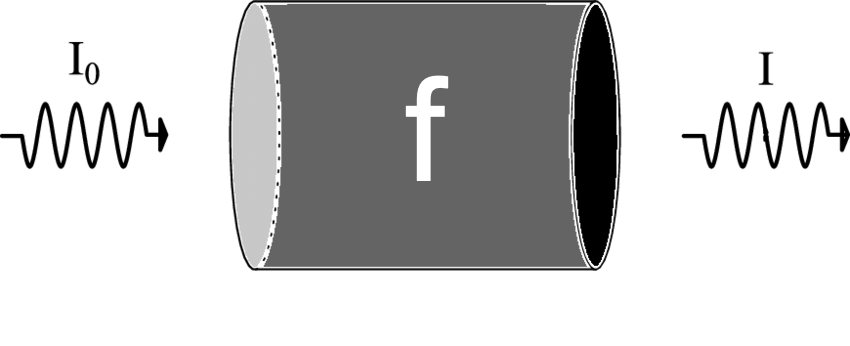
\includegraphics[scale = 0.4]{loiBeerLambert.png}
        \caption{Loi de Beer-Lambert}
    \end{figure}
\end{frame}

\begin{frame}{Lien avec la santé}
    \begin{beamerboxesrounded}{Loi de Beer-Lambert}
    Soit $(u, \theta)$ le couple caractérisant la droite passant par le point $(u \cos(\theta), u \sin(\theta))$ et orthogonale au vecteur $^t (\cos(\theta), \sin(\theta))$
    $$I(u,\theta) = I_0(u,\theta) \cdot \exp\left({- \int_{-\infty}^{+\infty} f(u \cos{\theta} - v \sin{\theta}, u \sin{\theta} + v \cos{\theta}) \dd v}\right)$$
    \pause
    ou encore : 
    $$I(u,\theta) = I_0(u,\theta) \cdot \exp\left(-R[f](u,\theta)\right)$$
    \end{beamerboxesrounded}
    
\end{frame}
\section{La reconstruction tomographique}
\subsection{Utilisation des sinogrammes}

\begin{frame}{Utilisation des sinogrammes}
    \begin{beamerboxesrounded}{Définition}
        On appelle sinogramme la représentation des valeurs de la fonction \\$(u,\theta) \mapsto R[f](u,\theta)$ dans le plan d'axes $u$ et $\theta$. 
    \end{beamerboxesrounded}
    \begin{figure}[t]
        \centering
        \begin{subfigure}[b]{0.42\textwidth}
            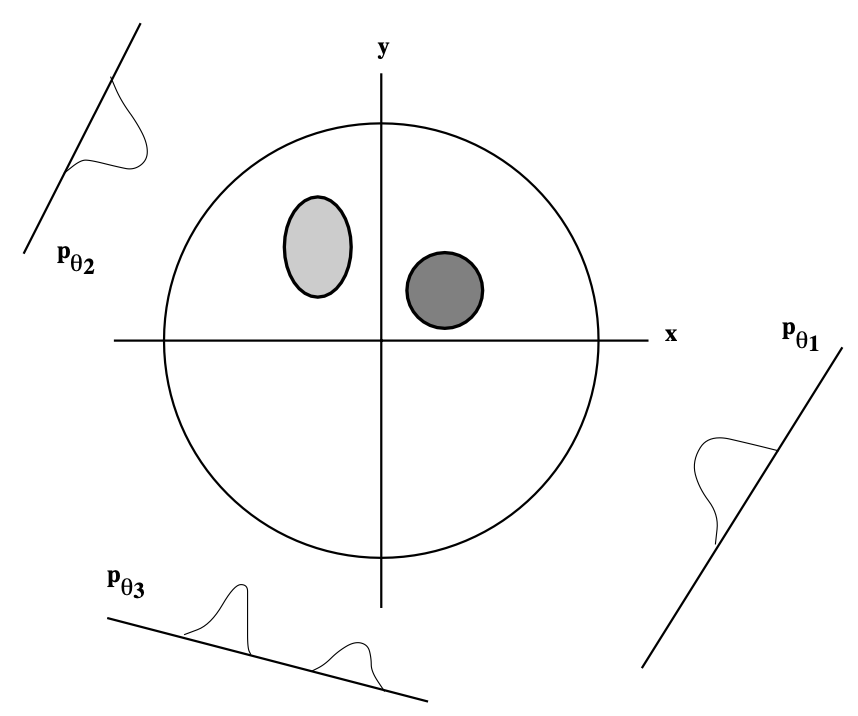
\includegraphics[width=\textwidth]{projectionStep3.png}
        \end{subfigure}
        \qquad \qquad 
        \begin{subfigure}[b]{0.42\textwidth}
            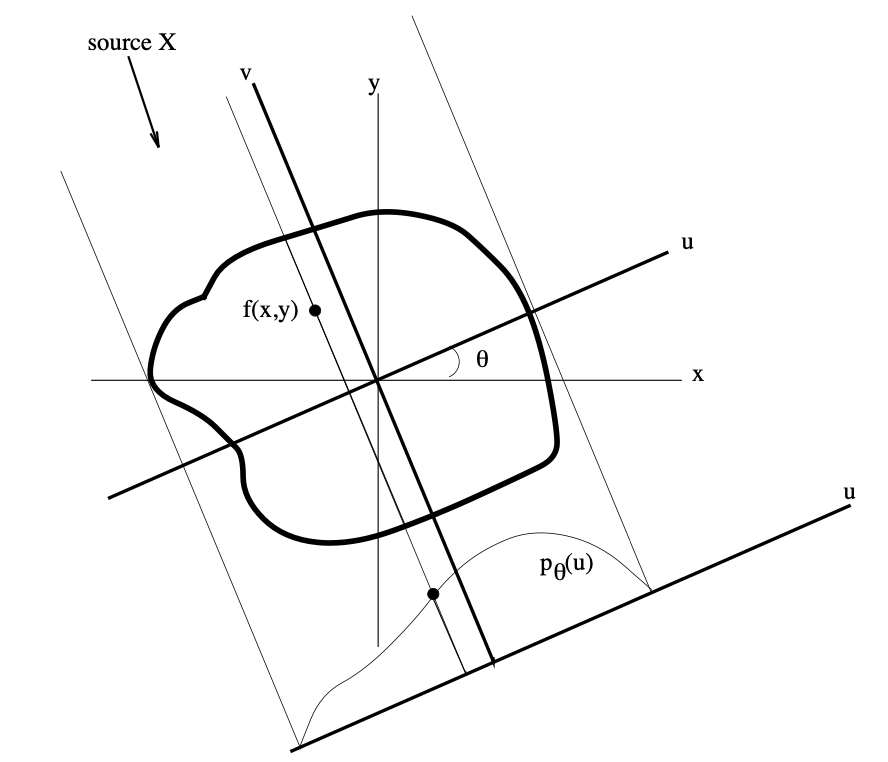
\includegraphics[width=\textwidth]{projection2.png}
        \end{subfigure}
        \caption{Projection}
    \end{figure}
\end{frame}

\begin{frame}{Utilisation des sinogrammes}
    \begin{figure}[t]
        \centering
        \begin{subfigure}[b]{0.45\textwidth}
            
\includegraphics[width=\textwidth]{image-reduite.png}
            \caption{Objet à reconstruire}
        \end{subfigure}
        \pause
        \qquad \qquad 
        \begin{subfigure}[b]{0.2\textwidth}
            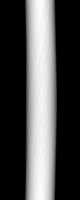
\includegraphics[width=\textwidth]{sino_rond.png}
            \caption{Sinogramme de l'objet}
        \end{subfigure}
    \end{figure}
\end{frame}

% \begin{frame}{La reconstruction - Utilisation des sinogrammes}
%     \begin{figure}[t]
%         \centering
%         \begin{subfigure}[b]{0.45\textwidth}
%             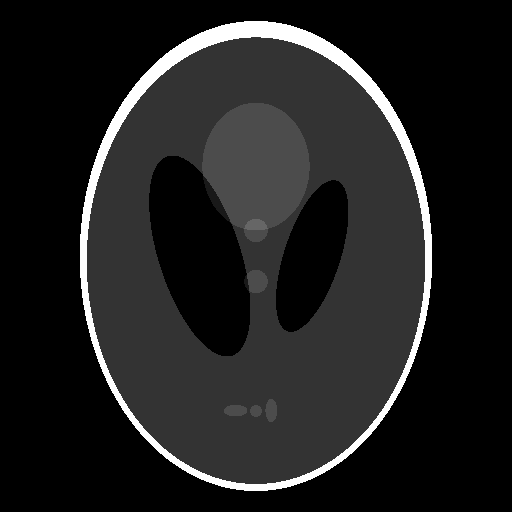
\includegraphics[width=\textwidth]{original.png}
%             \caption{Objet à reconstruire}
%         \end{subfigure}
%         \pause
%         \qquad \qquad 
%         \begin{subfigure}[b]{0.3\textwidth}
%             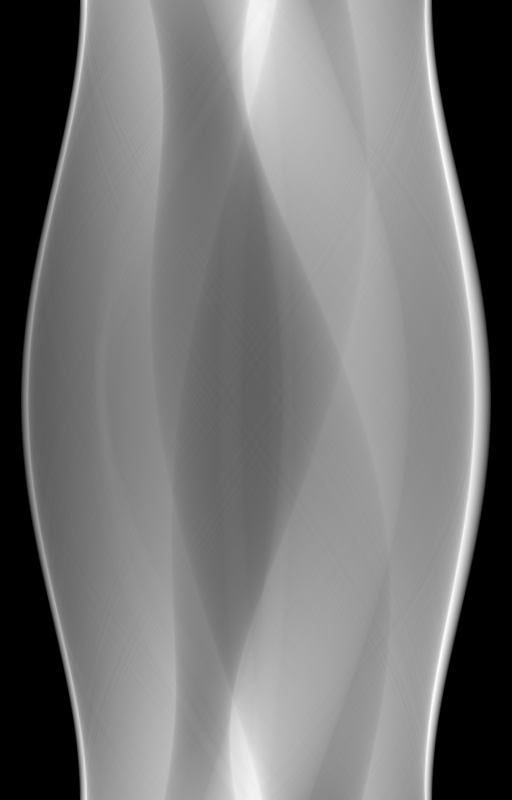
\includegraphics[width=\textwidth]{sinogram.png}
%             \caption{Sinogramme de l'objet}
%         \end{subfigure}
%     \end{figure}
% \end{frame}

\begin{frame}{Utilisation des sinogrammes}
    \begin{figure}[t]
        \centering
        \begin{subfigure}[b]{0.55\textwidth}
            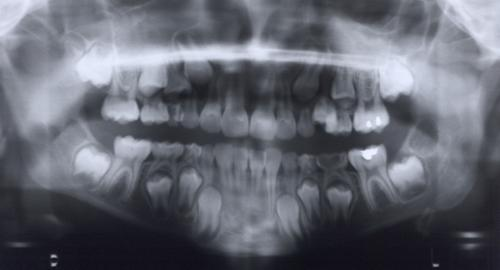
\includegraphics[width=\textwidth]{radio_dent.jpeg}
            \caption{Objet à reconstruire}
        \end{subfigure}
        \pause
        \qquad \qquad 
        \begin{subfigure}[b]{0.25\textwidth}
            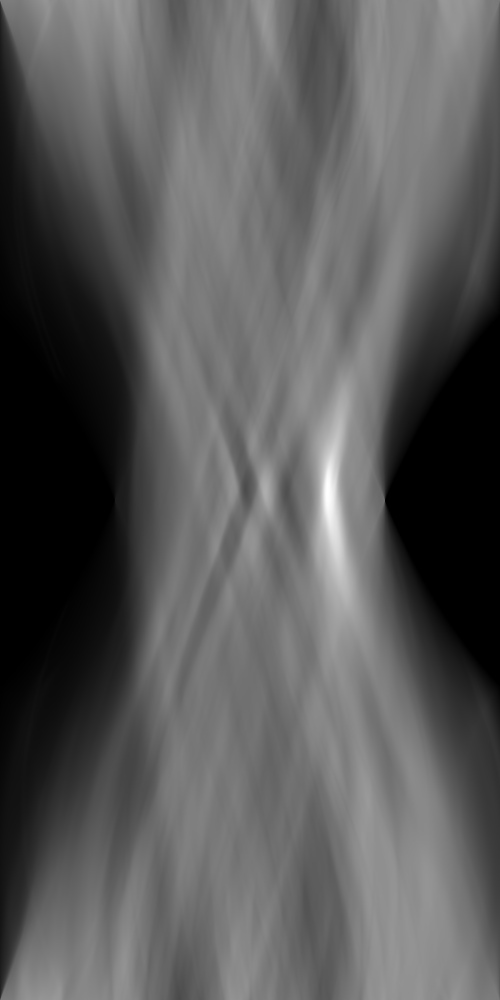
\includegraphics[width=\textwidth]{sino_dent.png}
            \caption{Sinogramme de l'objet}
        \end{subfigure}
    \end{figure}
\end{frame}

\begin{frame}{Utilisation des sinogrammes}
    \begin{figure}[t]
        \centering
        \begin{subfigure}[b]{0.35\textwidth}
            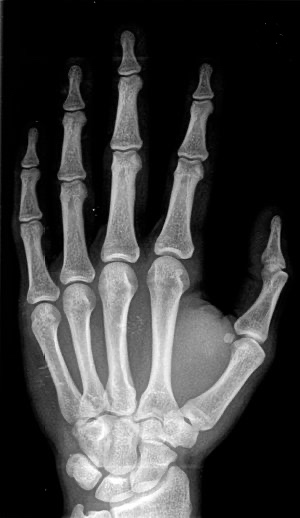
\includegraphics[width=\textwidth]{radio_main.jpeg}
            \caption{Objet à reconstruire}
        \end{subfigure}
        \pause
        \qquad \qquad 
        \begin{subfigure}[b]{0.22\textwidth}
            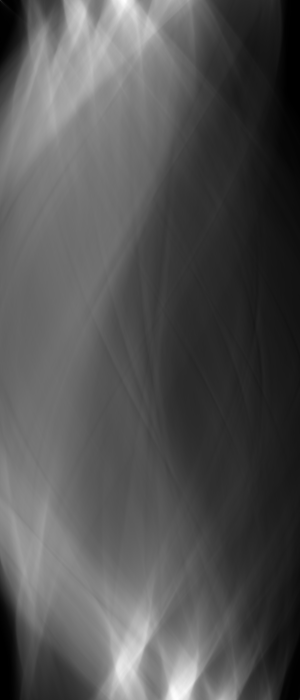
\includegraphics[width=\textwidth]{sino_main.png}
            \caption{Sinogramme de l'objet}
        \end{subfigure}
    \end{figure}
\end{frame}

\subsection{La résolution analytique}
\subsubsection{La rétroprojection simple}

\begin{frame}{La reconstruction - Inversion analytique}
    \begin{beamerboxesrounded}{Théorème de la coupe centrale}
        Soient $\theta \in [0,\pi[$ et $u \in \R$ et $f : \R^2 \longrightarrow \R$ la fonction caractéristique de notre objet. En notant $p_{\theta} : t \in \R \longmapsto R[f](t,\theta)$ on a : 
    $$\widehat{p_{\theta}}(u) = \widehat{f}(u \cos \theta , u \sin \theta)$$    
    où  $\; \widehat{.}\;$ est l'opérateur de transformée de Fourier.   
    \end{beamerboxesrounded}
    \begin{beamerboxesrounded}{Rétroprojection simple}
        Soit $f : \R^2 \longrightarrow \R$ la fonction caractéristique de notre objet. Pour $\theta \in \R$ on note $p_{\theta} : t \in \R \longmapsto R[f](t,\theta)$. On a alors : 
        $$\forall (x,y) \in \R^2, \quad f(x,y) = \int_{0}^{2\pi}\int_{\R^+} \widehat{p_{\theta}}(u) \mathrm{e}^{2i \pi u (x \cos \theta + y \sin \theta)} \; \dd u \; \dd \theta$$
    \end{beamerboxesrounded}

\end{frame}

% \begin{frame}{La reconstruction - Inversion analytique}
%     \begin{figure}[t]
%         \centering
%         \begin{subfigure}[b]{0.42\textwidth}
%             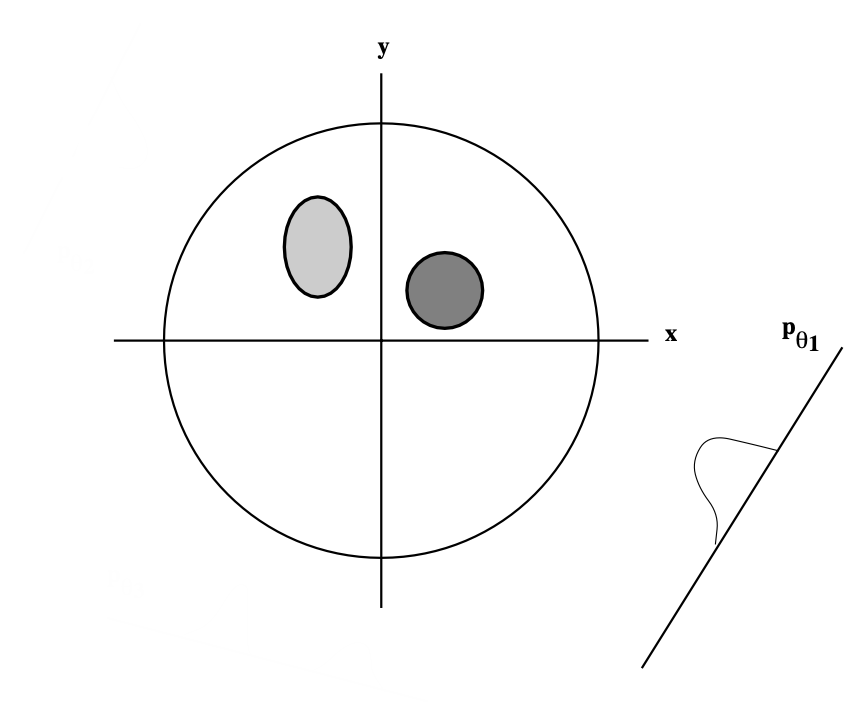
\includegraphics[width=\textwidth]{projectionStep1.png}
%         \end{subfigure}
%         \qquad \qquad 
%         \begin{subfigure}[b]{0.42\textwidth}
%             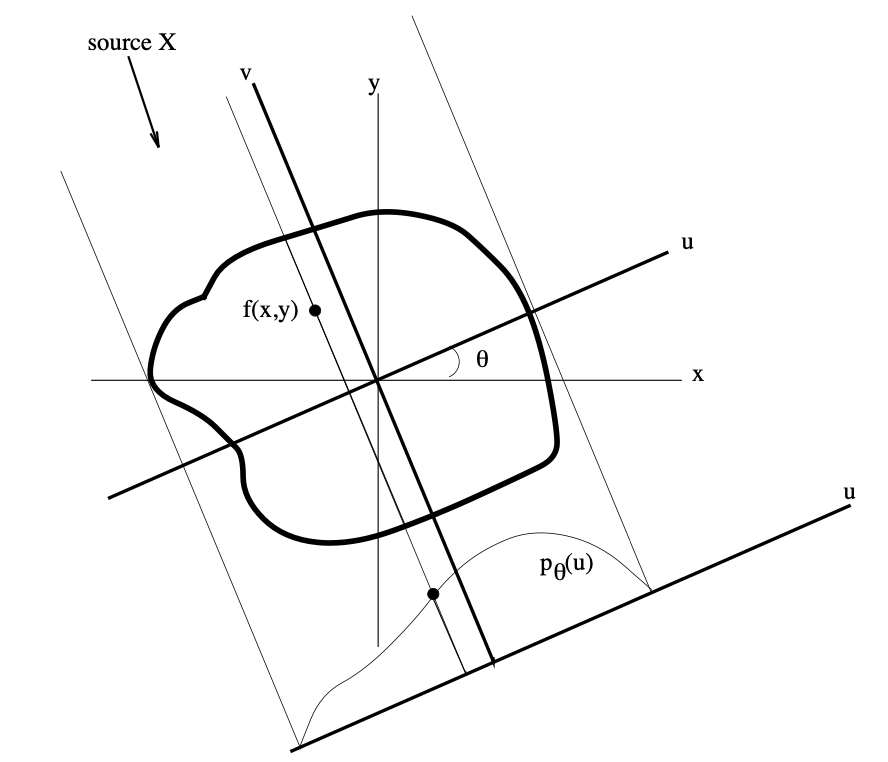
\includegraphics[width=\textwidth]{projection2.png}
%         \end{subfigure}
%         \caption{Projection}
%     \end{figure}
% \end{frame}

% \begin{frame}{La reconstruction - Inversion analytique}
%     \begin{figure}[t]
%         \centering
%         \begin{subfigure}[b]{0.42\textwidth}
%             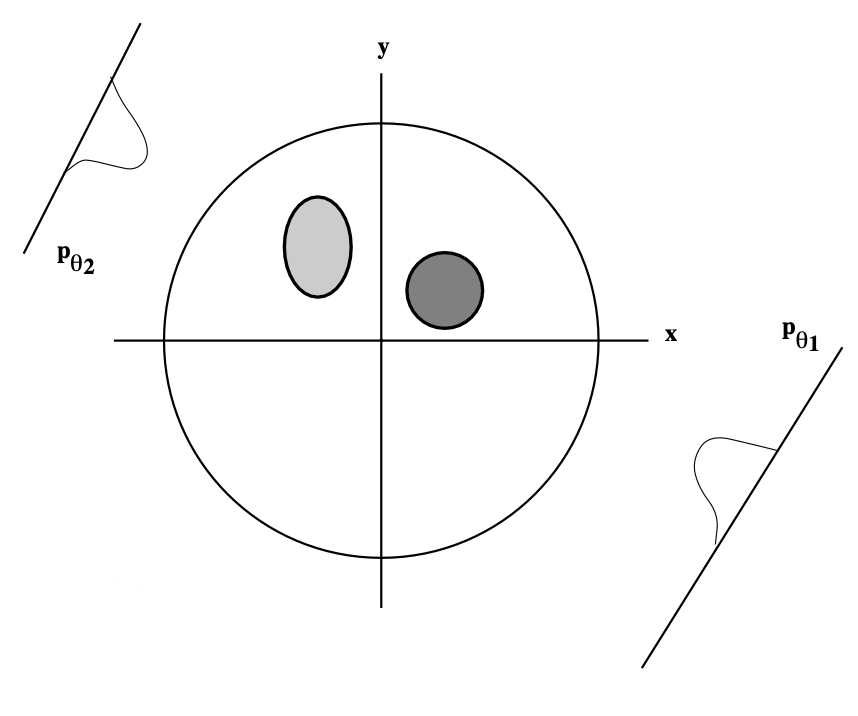
\includegraphics[width=\textwidth]{projectionStep2.png}
%         \end{subfigure}
%         \qquad \qquad 
%         \begin{subfigure}[b]{0.42\textwidth}
%             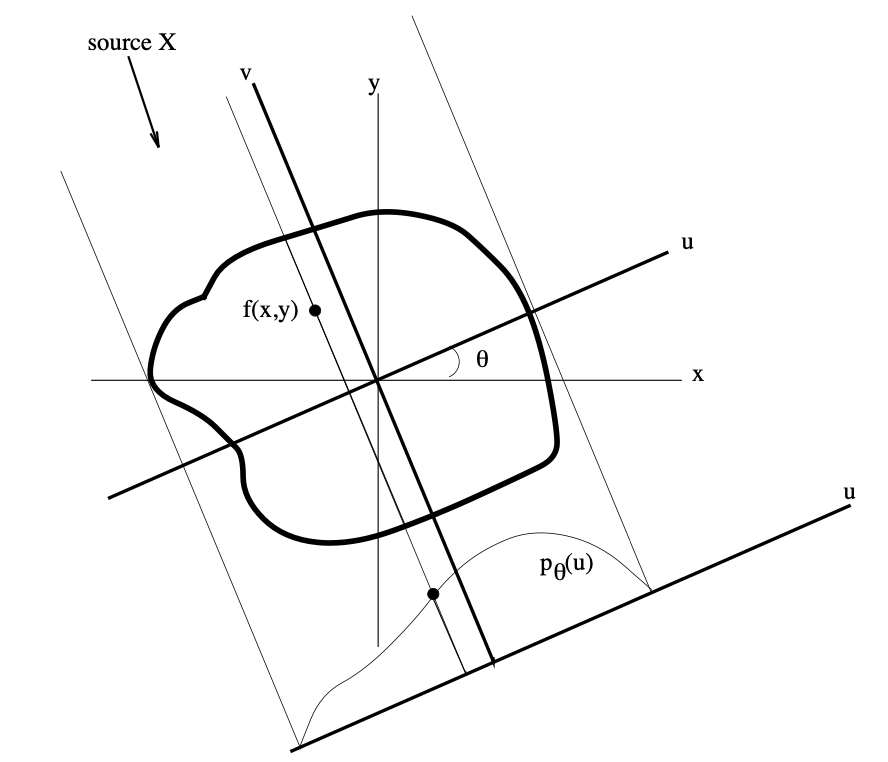
\includegraphics[width=\textwidth]{projection2.png}
%         \end{subfigure}
%         \caption{Projection}
%     \end{figure}
% \end{frame}

\begin{frame}{La reconstruction - Inversion analytique}
La rétroprojection simple (méthode naïve) : 
\begin{picture}(10,5)
    \put(0,3.2){\tiny objet à reconstruire }
    \put(0.3,2.65){$f(x,y)$}
    \pause
    \put(1.9, 2.7){\vector(1,0){1.5}}
    \put(2.1,2.8){\tiny projections}
    \put(3.7, 2.7){$\{p_{\theta}\}_{\theta}$}
    \pause
    \put(4.9, 2.7){\vector(1,0){2.5}}
    \put(5.6, 2.8){\tiny Fourier}
    \put(7.5, 2.7){$\{\widehat{p}_{\theta}\}_{\theta}$}
    \pause
    \put(8.6, 2.7){\vector(1,0){1.5}}
    \put(10.2, 2.65){$g(x,y)$}
    \put(10.2, 3.2){\tiny objet reconstruit}
\end{picture}
\pause 
Inconvénient : problème de flou $\rightarrow$ nécessité de la rétroprojection filtrée  
\end{frame}

\begin{frame}{La reconstruction - Inversion analytique}
    \begin{figure}[t]
        \centering
        \begin{subfigure}[b]{0.42\textwidth}
            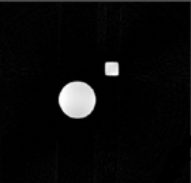
\includegraphics[width=\textwidth]{retrop.png}
        \end{subfigure}
        \qquad \qquad 
        \pause
        \begin{subfigure}[b]{0.42\textwidth}
            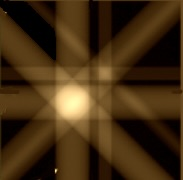
\includegraphics[width=\textwidth]{retrop_simple copie.jpeg}
        \end{subfigure}
        \caption{Rétroprojection simple}
    \end{figure}
\end{frame}

\begin{frame}{La reconstruction - Inversion analytique}
    $\rightarrow$ Nécessité de l'utilisation des filtres
    \begin{figure}[h]
        \centering
        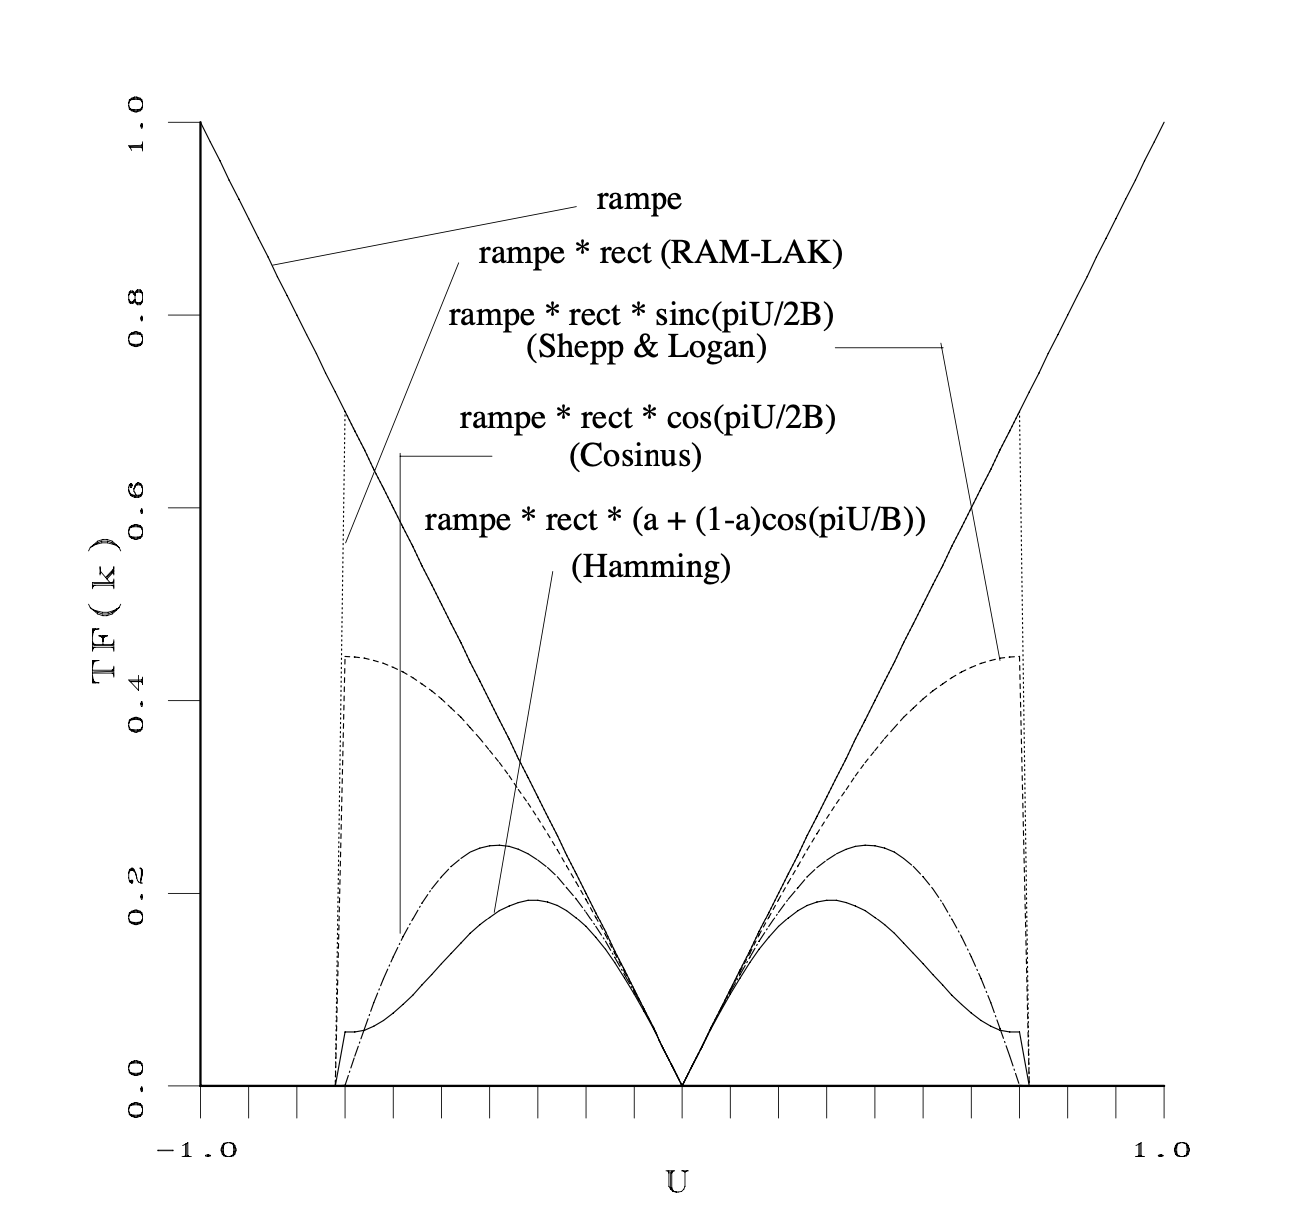
\includegraphics[scale = 0.3]{filtres.png}
        \caption{Quelques exemples de filtres}
    \end{figure}
\end{frame}

\subsubsection{La rétroprojection filtrée}
\begin{frame}{La reconstruction - Inversion analytique}
    \begin{beamerboxesrounded}{Rétroprojection filtrée}
        Soit $f : \R^2 \longrightarrow \R$ la fonction caractéristique de notre objet. Pour $\theta \in \R$ on note $p_{\theta} : t \in \R \longmapsto R[f](t,\theta)$. On a alors : 
        $$\forall (x,y) \in \R^2, \quad f(x,y) = \int_{0}^{2\pi}\int_{\R^+} \widehat{p_{\theta}}(u) \lvert u \rvert \mathrm{e}^{2i \pi u (x \cos \theta + y \sin \theta)} \; \dd u \; \dd \theta$$
    \end{beamerboxesrounded}
\end{frame}

\begin{frame}{La reconstruction - Inversion analytique}
    \begin{picture}(10,10)
        \put(0,8.2){\tiny objet à reconstruire }
        \put(0.3,7.65){$f(x,y)$}
        \pause
        \put(1.9, 7.7){\vector(1,0){1.5}}
        \put(2.1,7.8){\tiny projections}
        \put(3.7, 7.7){$\{p_{\theta}\}_{\theta}$}
        \pause
        \put(4.05,7.4){\vector(0,-1){1.5}}
        \put(3.35, 6.6){\tiny Fourier }
        \put(3.7, 5.3){$\{\widehat{p}_{\theta}\}_{\theta}$}
        \pause
        \put(4.9, 5.4){\vector(1,0){2.5}}
        \put(5.6, 5.6){\tiny Filtrage}
        \put(5.4, 4.9){$\lvert \nu \rvert \widehat{p}_{\theta}(\nu)$}
        \put(7.5, 5.3){$\{\tilde{\widehat{p}}_{\theta}\}_{\theta}$}
        \pause
        \put(4.9, 7.7){\vector(1,0){2.5}}
        \put(5.6, 7.2){\tiny Filtrage}
        \put(5.2, 7.9){$(p_{\theta} \ast k)(t)$}
        \put(7.5, 7.7){$\{\tilde{p}_{\theta}\}_{\theta}$}
        \pause
        \put(7.8,5.9){\vector(0,1){1.5}}
        \put(7.1,6.6){\tiny Fourier inverse}
        \pause
        \put(8.6, 7.7){\vector(1,0){1.5}}
        \put(10.2, 7.65){$g(x,y)$}
        \put(10.2, 8.2){\tiny objet reconstruit}
        \pause
        \put(8.5, 5.3){\vector(1,1){2}}
        \put(10, 6.2){\tiny Fourier inverse 2D}
    \end{picture}
\end{frame}

\begin{frame}{La reconstruction - Inversion analytique}
    \begin{figure}[t]
        \centering
        \begin{subfigure}[b]{0.42\textwidth}
            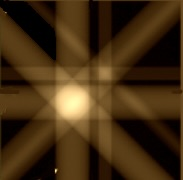
\includegraphics[width=\textwidth]{retrop_simple copie.jpeg}
            \caption{Rétroprojection simple}
        \end{subfigure}
        \qquad \qquad 
        \pause
        \begin{subfigure}[b]{0.42\textwidth}
            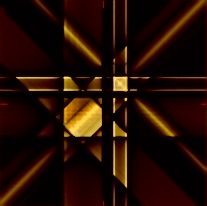
\includegraphics[width=\textwidth]{retrop_filtree copie.jpeg}
            \caption{Rétroprojection filtrée}
        \end{subfigure}
    \end{figure}
\end{frame}

\section{La résolution discrète}
\begin{frame}{La reconstruction - Inversion discrète}
    \begin{itemize}
        \item Nécessité de discrétiser les procédés pour les programmer en Python. 
        \item Deux méthodes : 
            \begin{itemize}
                \item La transformée de Fourier discrète
                \item La méthode ART ou méthode de Kaczmarz
            \end{itemize}
    \end{itemize}
\end{frame}
\subsection{Une première méthode : la transformée de Fourier discrète}
\begin{frame}{La reconstruction - Inversion discrète}
    \begin{beamerboxesrounded}{Transformée de Fourier discrète}
        Soit $f$ une fonction estimée aux points $(u_1, ... , u_N)$ on définit la transformée de Fourier discrète (TFD) de $f$ par la suite $(F(u_1), ... , F(u_N))$
        où : $$\forall k \in \iintervalle{1}{N}, \; F(u_k) = \sum_{j = 1}^N f(u_j)\exp\left(\frac{-2i\pi k j}{N}\right)$$
        Comme pour la transformée de Fourier on adapte la définition aux dimensions supérieures.
    \end{beamerboxesrounded}
    \begin{beamerboxesrounded}{Theorème de la coupe centrale}
        Soient $f$ la fonction caractéristique de notre objet, $\theta_k$, un angle échantillonné et $(u_l \cos \theta_k, u_l \sin \theta_k)$ un point d'une des droites d'échantillonnage. On a : 
        $$P_{\theta_k}(u_l) = F(u_l \cos \theta_k, u_l \sin \theta_k)$$
    \end{beamerboxesrounded}
\end{frame}

\subsection{Une deuxième méthode : reconstruction algébrique}

\begin{frame}{La reconstruction - Inversion discrète}
    \definecolor{yqyqyq}{rgb}{0.5,0.5,0.5}
    \definecolor{wwzzff}{rgb}{0.4,0.6,1}
    \definecolor{cqcqcq}{rgb}{0.2,0.2,0.2}
    \begin{tikzpicture}[line cap=round,line join=round,>=triangle 45,x=1cm,y=1cm]
        \draw [color=cqcqcq,, xstep=1cm,ystep=1cm] (-6.8,-6.87) grid (6.8,6.87);
        \fill[line width=2pt,color=wwzzff,fill=wwzzff,fill opacity=0.87] (-1.3529354846319104,2.44445741796992) -- (-0.4625870969263796,2.6670445148963022) -- (-0.12870645153680557,2.555750966433111) -- (0.4277612907791512,1.754437417498134) -- (0.18291548416013023,1.2870045139527309) -- (-0.24,1.131193546104263) -- (-0.6183980647748475,1.131193546104263) -- (-1.2639006458613573,0.7305367716367747) -- (-1.9094032269478673,0.574725803788307) -- (-2.287801291722718,0.9753825782557954) -- (-2.376836130493271,1.8879896756539636) -- (-2.0206967754110585,2.3109051598140904) -- cycle;
        \pause
        \draw (-3.88,3.59) node[anchor=north west] {$\text{pixel} \; j$};
        \draw [->,line width=2pt] (-3.02,2.75) -- (-1.64,1.75);
        \pause
        \draw [line width=2pt,color=yqyqyq,domain=-6.8:6.8] plot(\x,{(--11.63819573386923--2.870469434960631*\x)/4.836221722943288});
        \draw (1.06,3) node[anchor=north west] {$p_i$};
        \pause
        \draw [line width=2pt] (-1.9569867834843448,1.2449232752693837)-- (-0.9952740251500527,1.8157339692692045);
        \draw [->,line width=2pt] (-1.74,0.11) -- (-1.7739758447853289,1.3535467701986585);
        \draw (-1.92,0.07) node[anchor=north west] {longueur $\ell$ notée $R_{i,j}$};
    \end{tikzpicture}
\end{frame}

\begin{frame}{La reconstruction - Inversion discrète}  
    \begin{beamerboxesrounded}{Définition des matrices} 
        matrice de projection : $P = (p_j)_j$ qui recense les valeurs des projections
        matrice de rétroprojection : $R = (R_{i,j})_{i,j}$
    \end{beamerboxesrounded}  
    \pause
    La définition de la matrice $R$ peut varier selon l'appareil étudié. 
    On peut par exemple simplifier en définissant la matrice $R$ de la sorte : 
    $$\forall (i,j) \in \iintervalle{1}{N} \times \iintervalle{1}{M},R_{i,j} = \left\{
        \begin{array}{ll}
            1 & \mbox{si le rayon } i \mbox{ passe par le pixel } j  \\
            0 & \mbox{sinon.}
        \end{array}
    \right.$$ 
    \pause 
    \begin{beamerboxesrounded}{Théorème}
        L'image $F$ à reconstruire est solution du système matriciel $RF = P$
    \end{beamerboxesrounded}
    \pause
    En effet, par définition de la matrice de projection : 
    $$\forall i \in \iintervalle{1}{N}, p_i = \sum_{j = 1}^M R_{i,j} f(j)$$
\end{frame}

\begin{frame}{La reconstruction - Inversion discrète}
    \begin{beamerboxesrounded}{Reformulation du problème}
        $F$ est solution du système si et seulement si $F \in \bigcap_{i =1}^N \mathcal{H}_i$ où $\mathcal{H}_i = p_i + \{^t L_i\}^{\perp}$
    \end{beamerboxesrounded}
    On peut résoudre par la méthode dite de Kaczmarz : 
    \begin{itemize}
        \item on choisit $F_0 \in \R^M$
        \pause
        \item on projette orthogonalement $F_0$ sur $\mathcal{H}_1$ pour obtenir $F_1$
        \pause
        \item on projette orthogonalement $F_1$ sur $\mathcal{H}_2$ pour obtenir $F_2$
        \item \dots
        \pause
        \item on projette orthogonalement $F_{N-1}$ sur $\mathcal{H}_N$ pour obtenir $F_N$
        \pause
        \item puis on recommence à partir du vecteur $F_N \dots$
    \end{itemize}
\end{frame}

\begin{frame}{La reconstruction - Inversion discrète}
    \begin{beamerboxesrounded}{Expression de la suite}
        La suite est alors définie par récurrence par la formule : 
        $$\left\{ 
        \begin{array}{ll}
            & F_0 \in M_{M,1}(\R)\\
            & \forall n \in \N^{*}, F_{n+1}= F_n - \frac{\scal{F_n - q_{r(n)+1}}{N_{r(n)+1}}}{\norme{N_{r(n)+1}}^2}N_{r(n)+1}  
        \end{array}\right.$$
        où $r(n)$ est le reste de la division euclidienne de $n$ par $N$. 
    \end{beamerboxesrounded}
cette expression découle de l'expression du projeté orthogonal d'un vecteur $x$ sur un hyperplan $H = \{a\}^{\perp}$ : 
$$p_H(x) = x - \frac{\scal{x}{a}}{\norme{a}^2}a $$
\end{frame}

\begin{frame}{La reconstruction - Inversion discrète}
    \definecolor{uuuuuu}{rgb}{0.26666666666666666,0.26666666666666666,0.26666666666666666}
    \definecolor{ududff}{rgb}{0.30196078431372547,0.30196078431372547,1}
    \definecolor{cqcqcq}{rgb}{0.7529411764705882,0.7529411764705882,0.7529411764705882}
    \begin{tikzpicture}[line cap=round,line join=round,>=triangle 45,x=1cm,y=1cm]
    \draw [color=cqcqcq,, xstep=0.5cm,ystep=0.5cm] (-6.825738728170894,-3.323643197569457) grid (7.179318629864831,5.802748875211437);
    \clip(-6.825738728170894,-3.323643197569457) rectangle (7.179318629864831,5.802748875211437);
    \draw [line width=1pt,domain=-6.825738728170894:7.179318629864831] plot(\x,{(--16.872505481862348--3.2990555973059905*\x)/8.379958609883893});
    \draw [line width=1pt,domain=-6.825738728170894:7.179318629864831] plot(\x,{(--13.86462588822425-7.815411248291108*\x)/-5.733656470634804});
    \draw [line width=1pt,domain=-6.825738728170894:7.179318629864831] plot(\x,{(-16.872505481862348-3.2990555973059905*\x)/-8.379958609883893});
    \draw (-6,0.5) node[anchor=north west] {$\mathcal{H}_1$};
    \draw (0.9,-1) node[anchor=north west] {$\mathcal{H}_2$};
    \pause
    \draw[color=ududff] (-4.48860034926011,2.919093346859538) node {$F_{0}$};
    \draw [fill=ududff] (-4.58474,2.7017) circle (2.5pt);
    \pause 
    \draw [line width=1pt] (-4.58474,2.7017)-- (-3.7349172900658614,0.5430582539188338);
    \draw [fill=ududff] (-3.7349172900658614,0.5430582539188338) circle (2pt);
    \draw[color=ududff] (-3.67104623952706,0.8130028685254858) node {$F_{1}$};
    \pause
    \draw [line width=1pt] (-3.7349172900658614,0.5430582539188338)-- (0.10545370652402351,-2.2743709656952342);
    \draw [fill=ududff] (0.10545370652402351,-2.2743709656952342) circle (2pt);
    \draw[color=ududff] (0.13,-1.9) node {$F_{2}$};   
    \pause
    \draw [line width=1pt] (-1.3702205530839788,1.474001516200577)-- (0.10545370652402351,-2.2743709656952342);
    \draw [fill=ududff] (-1.3702205530839788,1.474001516200577) circle (2pt);
    \draw[color=ududff] (-1.4316588954756626,1.7638538439758806) node {$F_{3}$};
    \pause
    \draw [line width=1pt] (-1.3702205530839788,1.474001516200577)-- (1.3768577222169673,-0.541350283995937);
    \draw [line width=1pt] (0.3212845227553587,2.1399199948118426)-- (1.3768577222169673,-0.541350283995937);
    \draw [line width=1pt] (0.3212845227553587,2.1399199948118426)-- (2.2863131768440894,0.6983068922432208);
    \draw [line width=1pt] (1.5312449277593612,2.6162620428428394)-- (2.2863131768440894,0.6983068922432208);
    \draw [line width=1pt] (1.5312449277593612,2.6162620428428394)-- (2.936861085881669,1.585053329160751);
    \draw [line width=1pt] (2.936861085881669,1.585053329160751)-- (2.3967487932745164,2.9569970637354195);
    \draw [line width=1pt] (2.3967487932745164,2.9569970637354195)-- (3.4022083217467656,2.2193571177061076);
    \draw [line width=1pt] (3.4022083217467656,2.2193571177061076)-- (3.015857433626426,3.2007302276301);
    \draw [line width=1pt] (3.015857433626426,3.2007302276301)-- (3.7350785791389494,2.6730846765803147);
    \draw [line width=1pt] (3.7350785791389494,2.6730846765803147)-- (3.458715662029889,3.3750764249375953);
    \draw [line width=1pt] (3.458715662029889,3.3750764249375953)-- (3.9731859529806637,2.9976431947535453);
    \draw [line width=1pt] (3.9731859529806637,2.9976431947535453)-- (3.775499175749186,3.499789024691639);
    \draw [line width=1pt] (3.775499175749186,3.499789024691639)-- (4.143507933448267,3.22980504972257);
    \draw [fill=ududff] (1.3768577222169673,-0.541350283995937) circle (2pt);
    \draw[color=ududff] (1.7,-0.4844199577900065) node {$F_{4}$};
    \draw [fill=ududff] (0.3212845227553587,2.1399199948118426) circle (2pt);
    \draw[color=ududff] (0.29231390113533406,2.394792341704647) node {$F_{5}$};
    \draw [fill=ududff] (2.2863131768440894,0.6983068922432208) circle (2pt);
    \draw[color=ududff] (2.55,0.7152518336660993) node {$F_{6}$};
    \draw [fill=ududff] (4.57147,3.81315) circle (2pt);
    \draw[color=ududff] (4.557813604090376,4.012127645741768) node {$F$};
    \draw [fill=ududff] (1.5312449277593612,2.6162620428428394) circle (2pt);
    \draw[color=ududff] (1.509758608020419,2.892433973716069) node {$F_{7}$};
    \draw [fill=ududff] (2.936861085881669,1.585053329160751) circle (2pt);
    \draw[color=ududff] (3.3,1.5772382319715976) node {$F_{8}$};
    \draw [fill=ududff] (2.3967487932745164,2.9569970637354195) circle (2pt);
    \draw[color=ududff] (2.327312717753469,3.247892282295656) node {$F_{9}$};
    \draw [fill=ududff] (3.4022083217467656,2.2193571177061076) circle (2pt);
    \draw[color=ududff] (3.8,2.1992902719858747) node {$F_{10}$};
    \draw [fill=ududff] (3.015857433626426,3.2007302276301) circle (2pt);
    \draw[color=ududff] (2.9404783000532566,3.478940182872387) node {$F_{11}$};
    \draw [fill=ududff] (3.7350785791389494,2.6730846765803147) circle (2pt);
    \draw[color=ududff] (4.4,3) node {$F_{14}$};
    \draw [fill=ududff] (3.458715662029889,3.3750764249375953) circle (2pt);
    \draw [fill=ududff] (3.9731859529806637,2.9976431947535453) circle (2pt);
    \draw[color=ududff] (4.6,3.3) node {$F_{16}$};
    \draw [fill=ududff] (3.775499175749186,3.499789024691639) circle (2pt);
    \draw [fill=ududff] (4.143507933448267,3.22980504972257) circle (2pt);
    \draw [fill=ududff] (3.7754991757491845,3.4997890246916397) circle (2pt);
    \draw[color=ududff] (3.820237613787734,3.827760998878098) node {$F_{15}$};
    \draw [fill=ududff] (3.458715662029889,3.3750764249375953) circle (2pt);
    \draw[color=ududff] (3.420347016635699,3.647782879447691) node {$F_{13}$};
    \draw [fill=ududff] (3.73507857913895,2.6730846765803142) circle (2pt);
    \draw[color=ududff] (4.2,2.6969319039972963) node {$F_{12}$};
    \end{tikzpicture}
\end{frame}

\section{Les résultats obtenus avec les codes Python}
\begin{frame}{Résultats - première méthode}
    Reconstruction de la main (155 400 pixels) : 
    \begin{figure}[t]
        \centering
        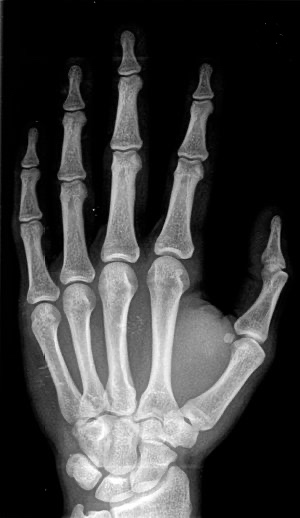
\includegraphics[scale = 0.35]{radio_main.jpeg}
        \caption{Radiographie originale}
    \end{figure}
\end{frame}

\begin{frame}{Résultats - première méthode}
    \begin{figure}[t]
        \centering
        \begin{subfigure}[b]{0.42\textwidth}
            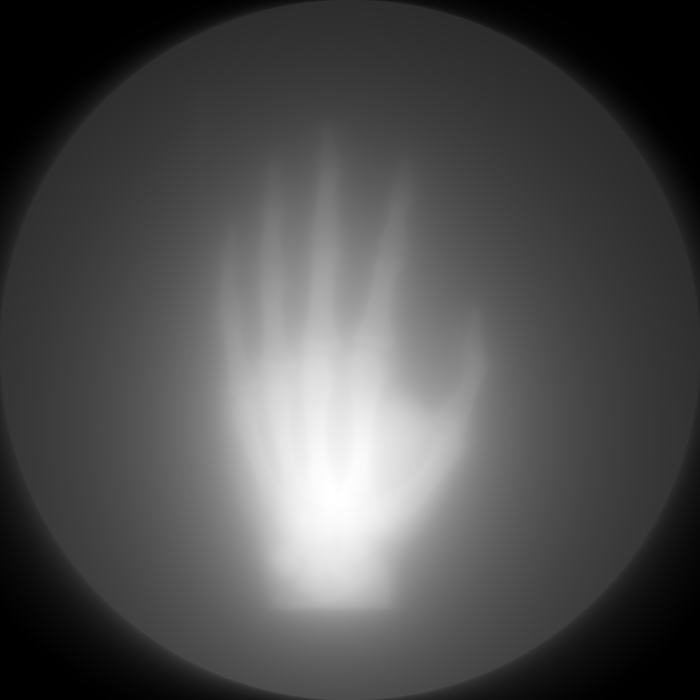
\includegraphics[width=\textwidth]{mainSansFFT.png}
            \caption{Sans transformée de Fourier}
        \end{subfigure}
        \qquad \qquad 
        \pause
        \begin{subfigure}[b]{0.42\textwidth}
            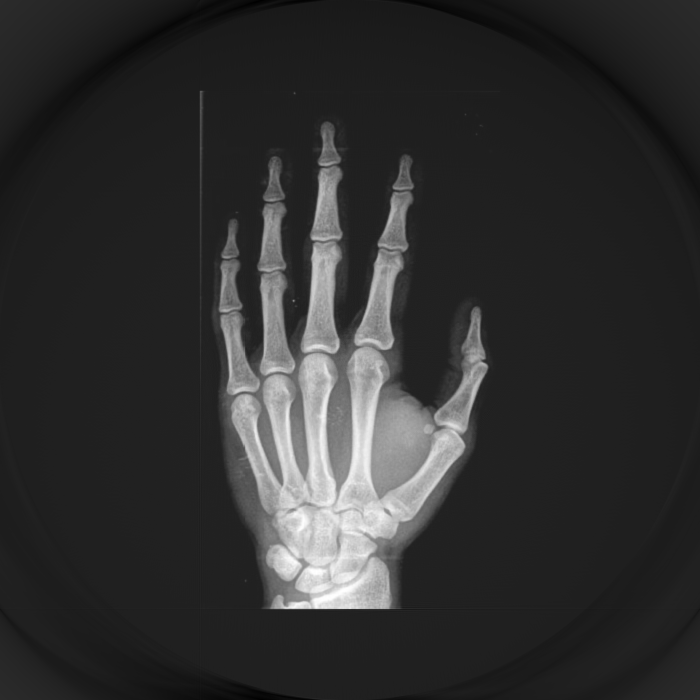
\includegraphics[width=\textwidth]{mainAvecFFT.png}
            \caption{Avec transformée de Fourier}
        \end{subfigure}
    \end{figure}
\end{frame}

\begin{frame}{Résultats - première méthode}
    Reconstruction de la mâchoire (135 000 pixels) : 
    \begin{figure}[t]
        \centering
        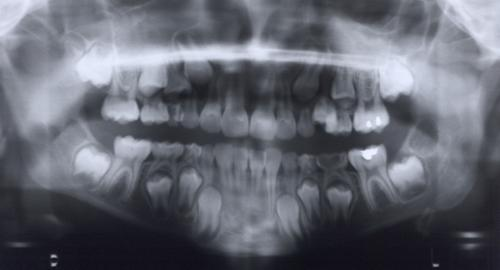
\includegraphics[scale = 0.35]{radio_dent.jpeg}
        \caption{Radiographie originale}
    \end{figure}
\end{frame}

\begin{frame}{Résultats - première méthode}
    \begin{figure}[t]
        \centering
        \begin{subfigure}[b]{0.42\textwidth}
            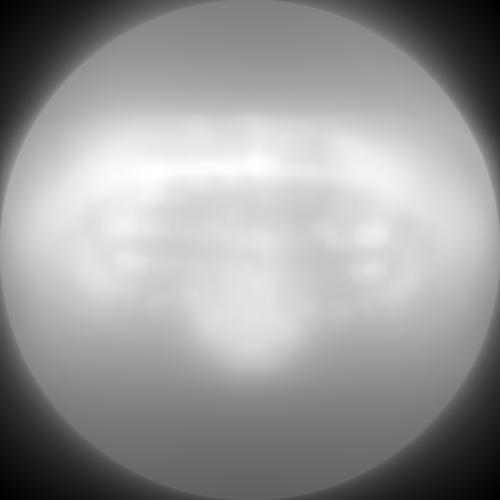
\includegraphics[width=\textwidth]{dentsSansFFT.png}
            \caption{Sans transformée de Fourier}
        \end{subfigure}
        \qquad \qquad 
        \pause
        \begin{subfigure}[b]{0.42\textwidth}
            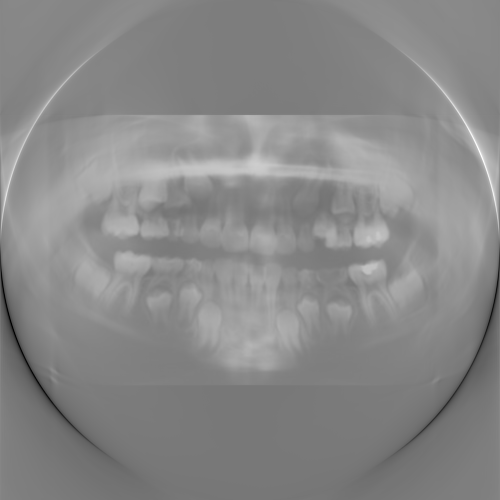
\includegraphics[width=\textwidth]{dentsAvecFFT.png}
            \caption{Avec transformée de Fourier}
        \end{subfigure}
    \end{figure}
\end{frame}

\begin{frame}{Résultats - première méthode}
    Reconstruction du genou (1 675 500 pixels) : 
    \begin{figure}[t]
        \centering
        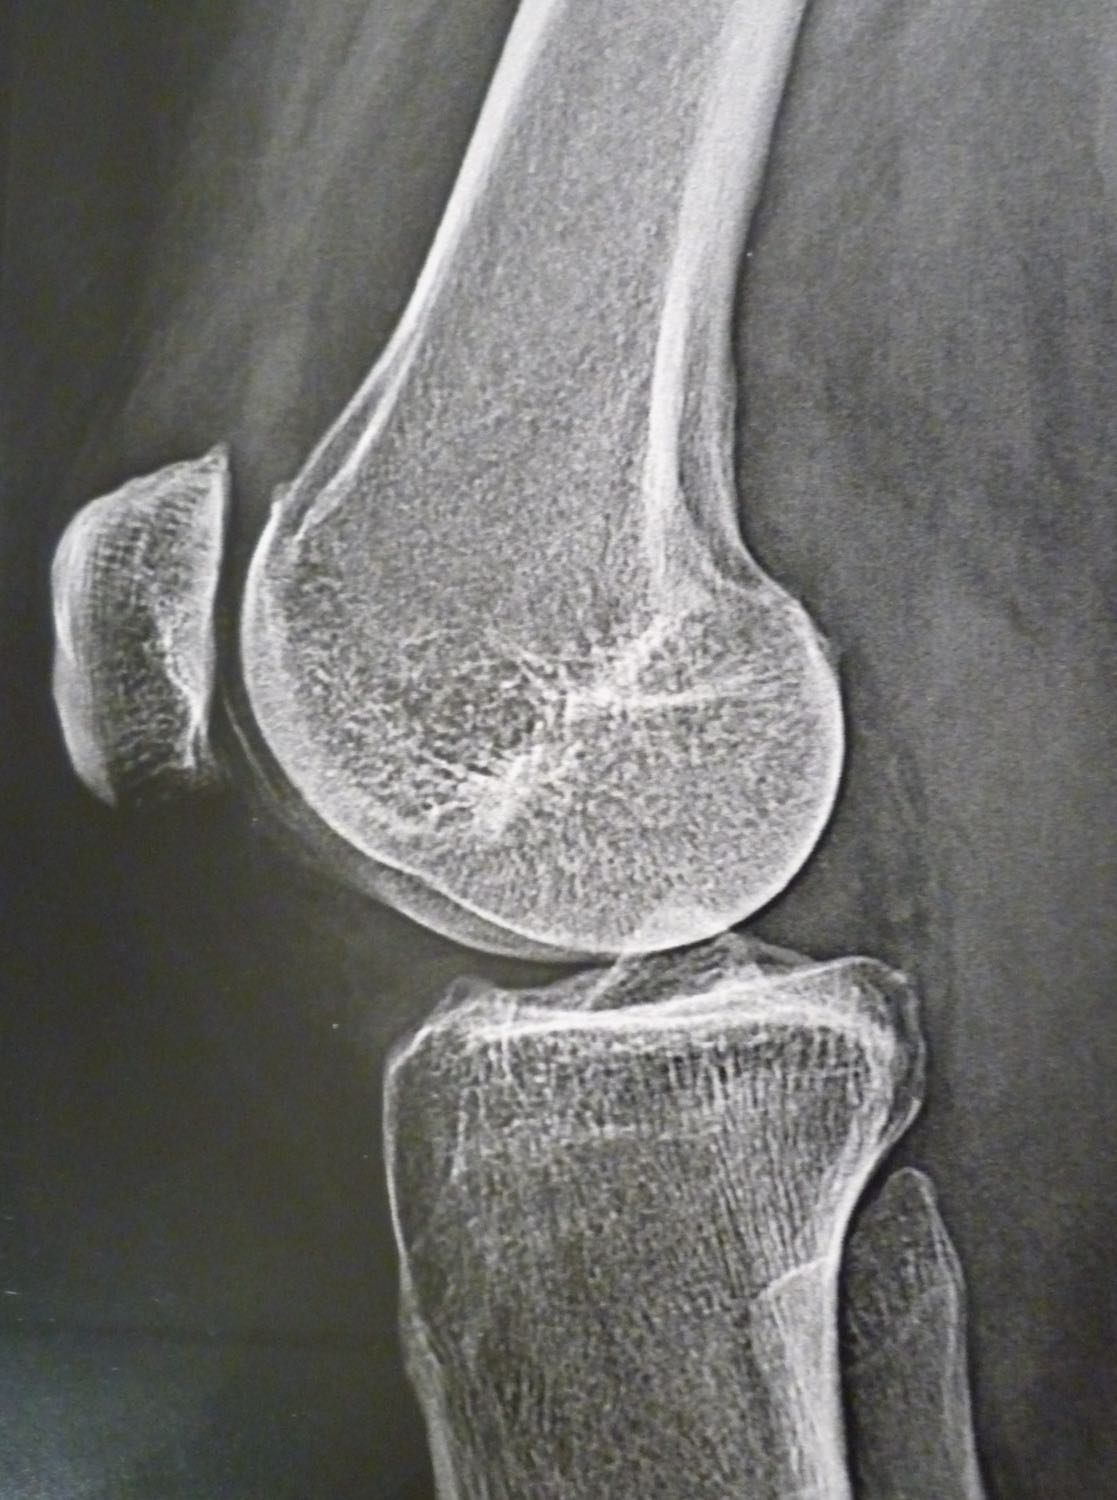
\includegraphics[scale = 0.1]{radio_genou.jpeg}
    \end{figure}
\end{frame}

\begin{frame}{Résultats - première méthode}
    \begin{figure}[t]
        \centering
        \begin{subfigure}[b]{0.42\textwidth}
            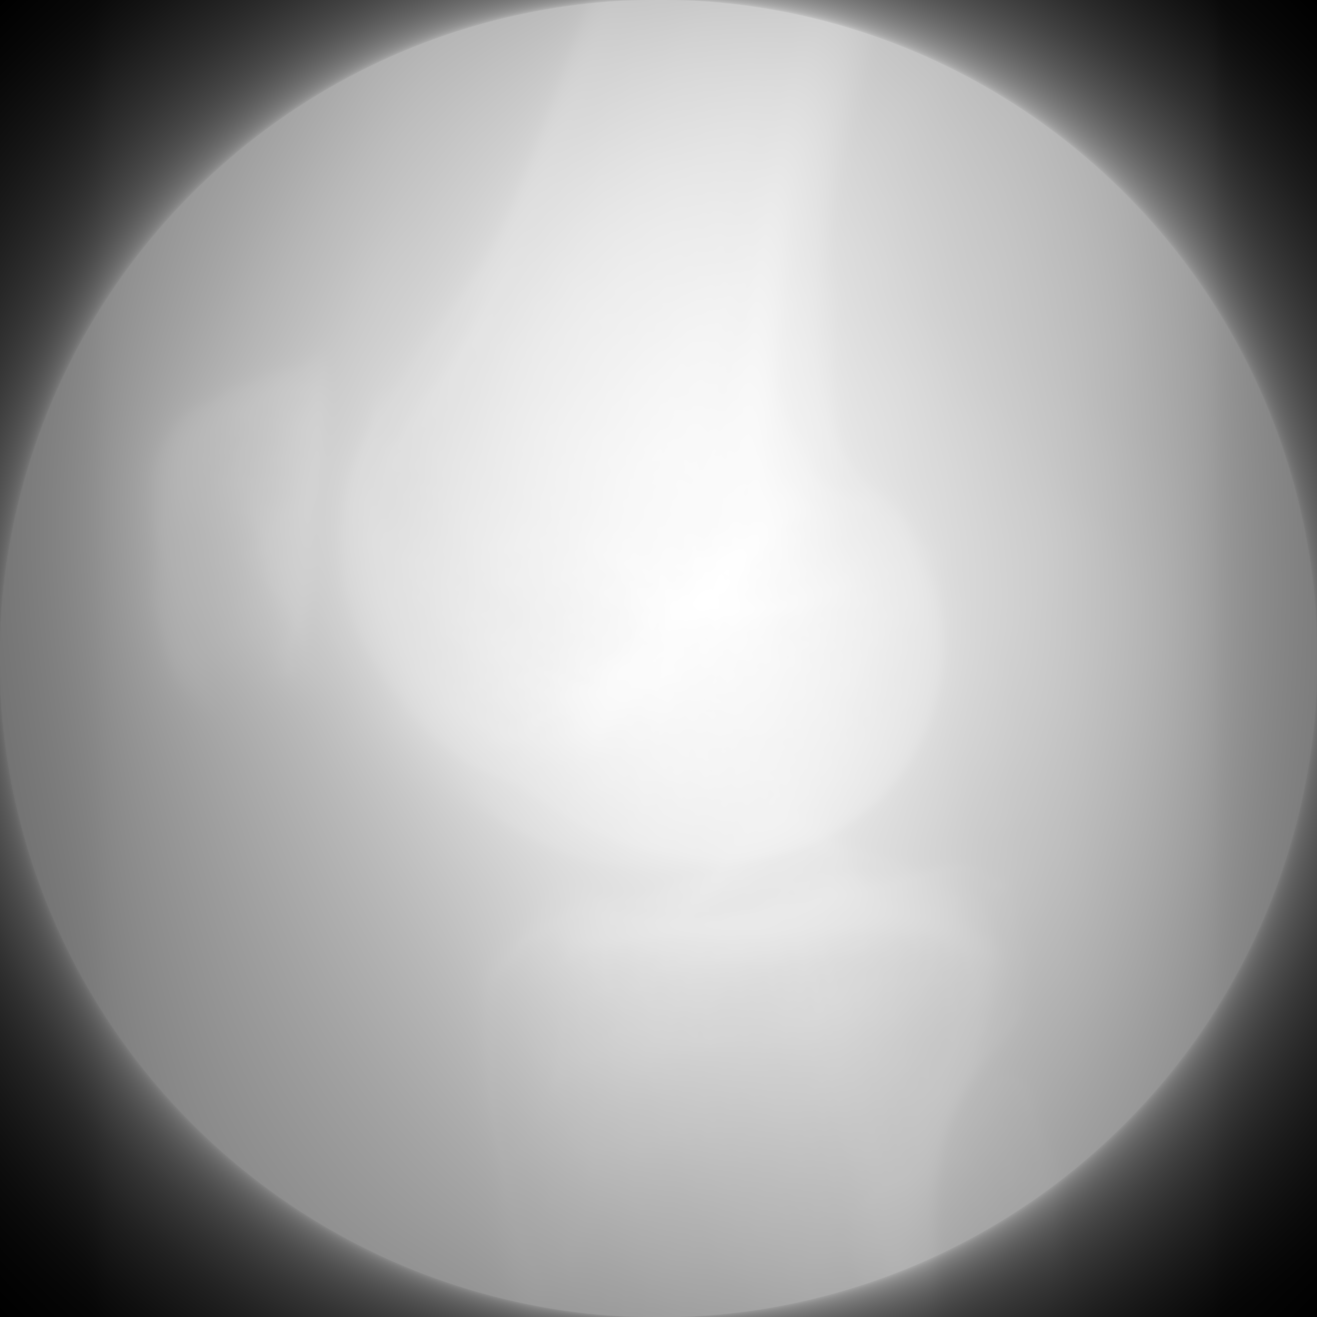
\includegraphics[width=\textwidth]{genouSansFFT.png}
            \caption{Sans transformée de Fourier}
        \end{subfigure}
        \qquad \qquad 
        \pause
        \begin{subfigure}[b]{0.42\textwidth}
            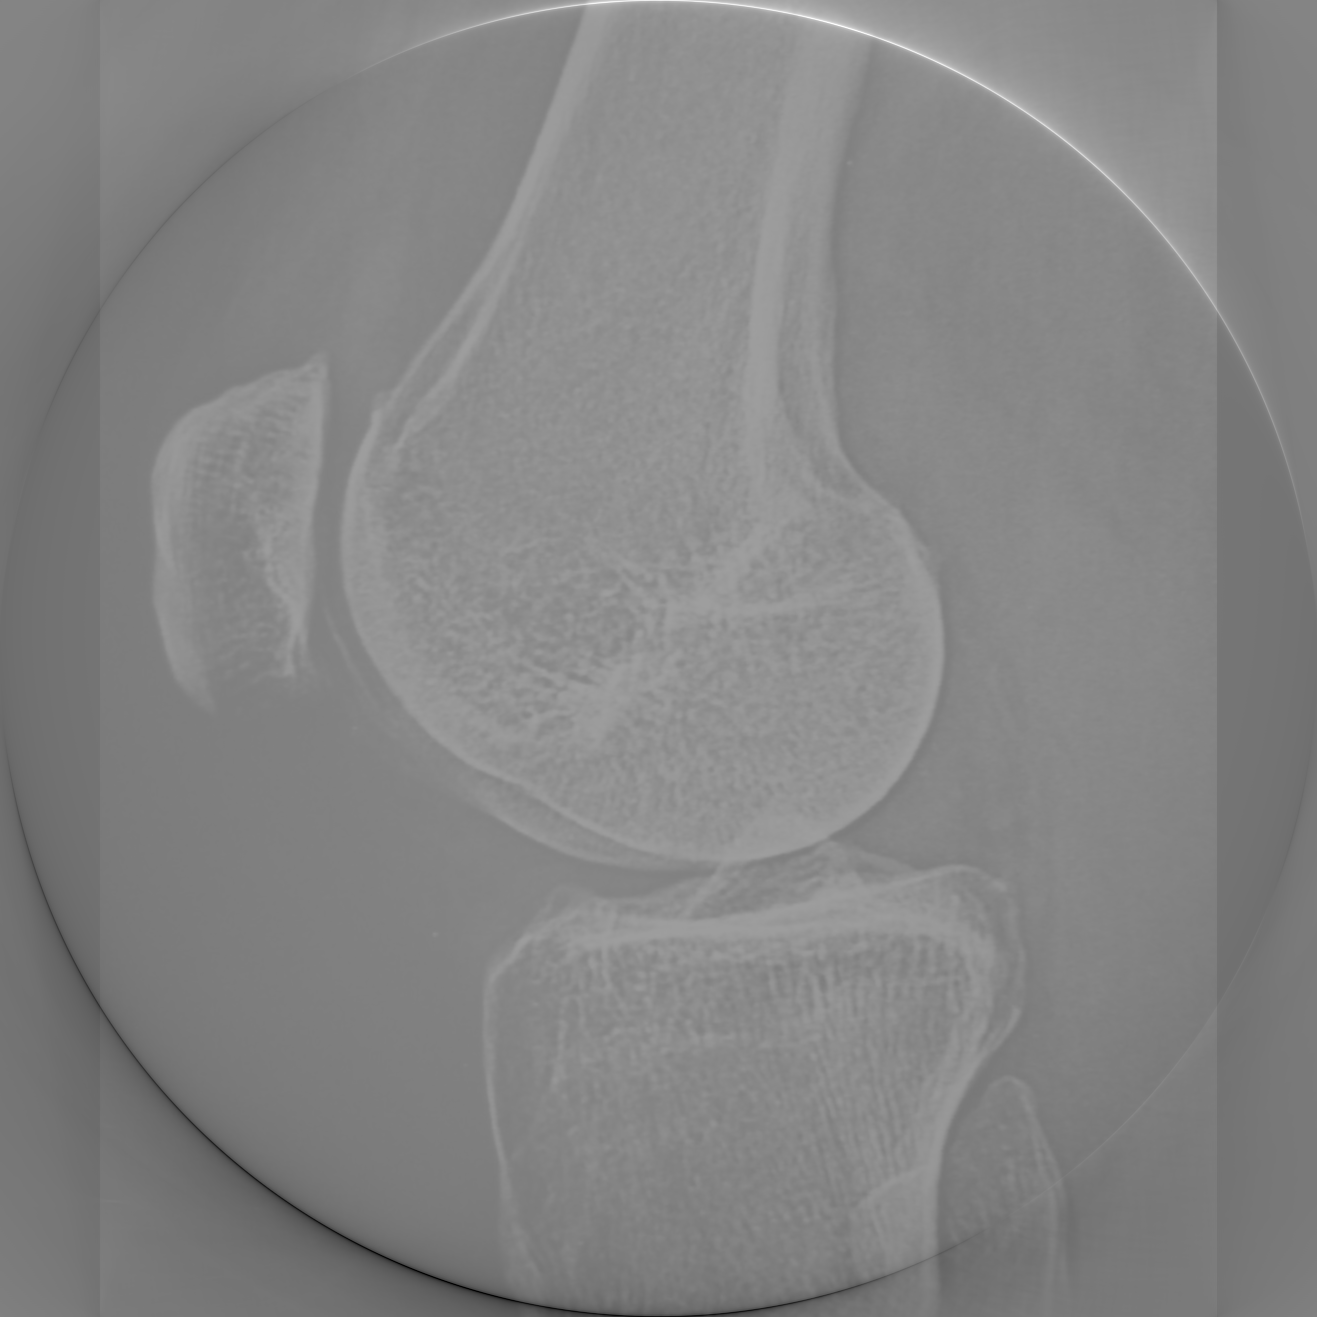
\includegraphics[width=\textwidth]{genouAvecFFT.png}
            \caption{Avec transformée de Fourier}
        \end{subfigure}
    \end{figure}
\end{frame}

\begin{frame}{Résultats - première méthode}
    Reconstruction du thorax (5 095 242 pixels) : 
    \begin{figure}
        \centering 
        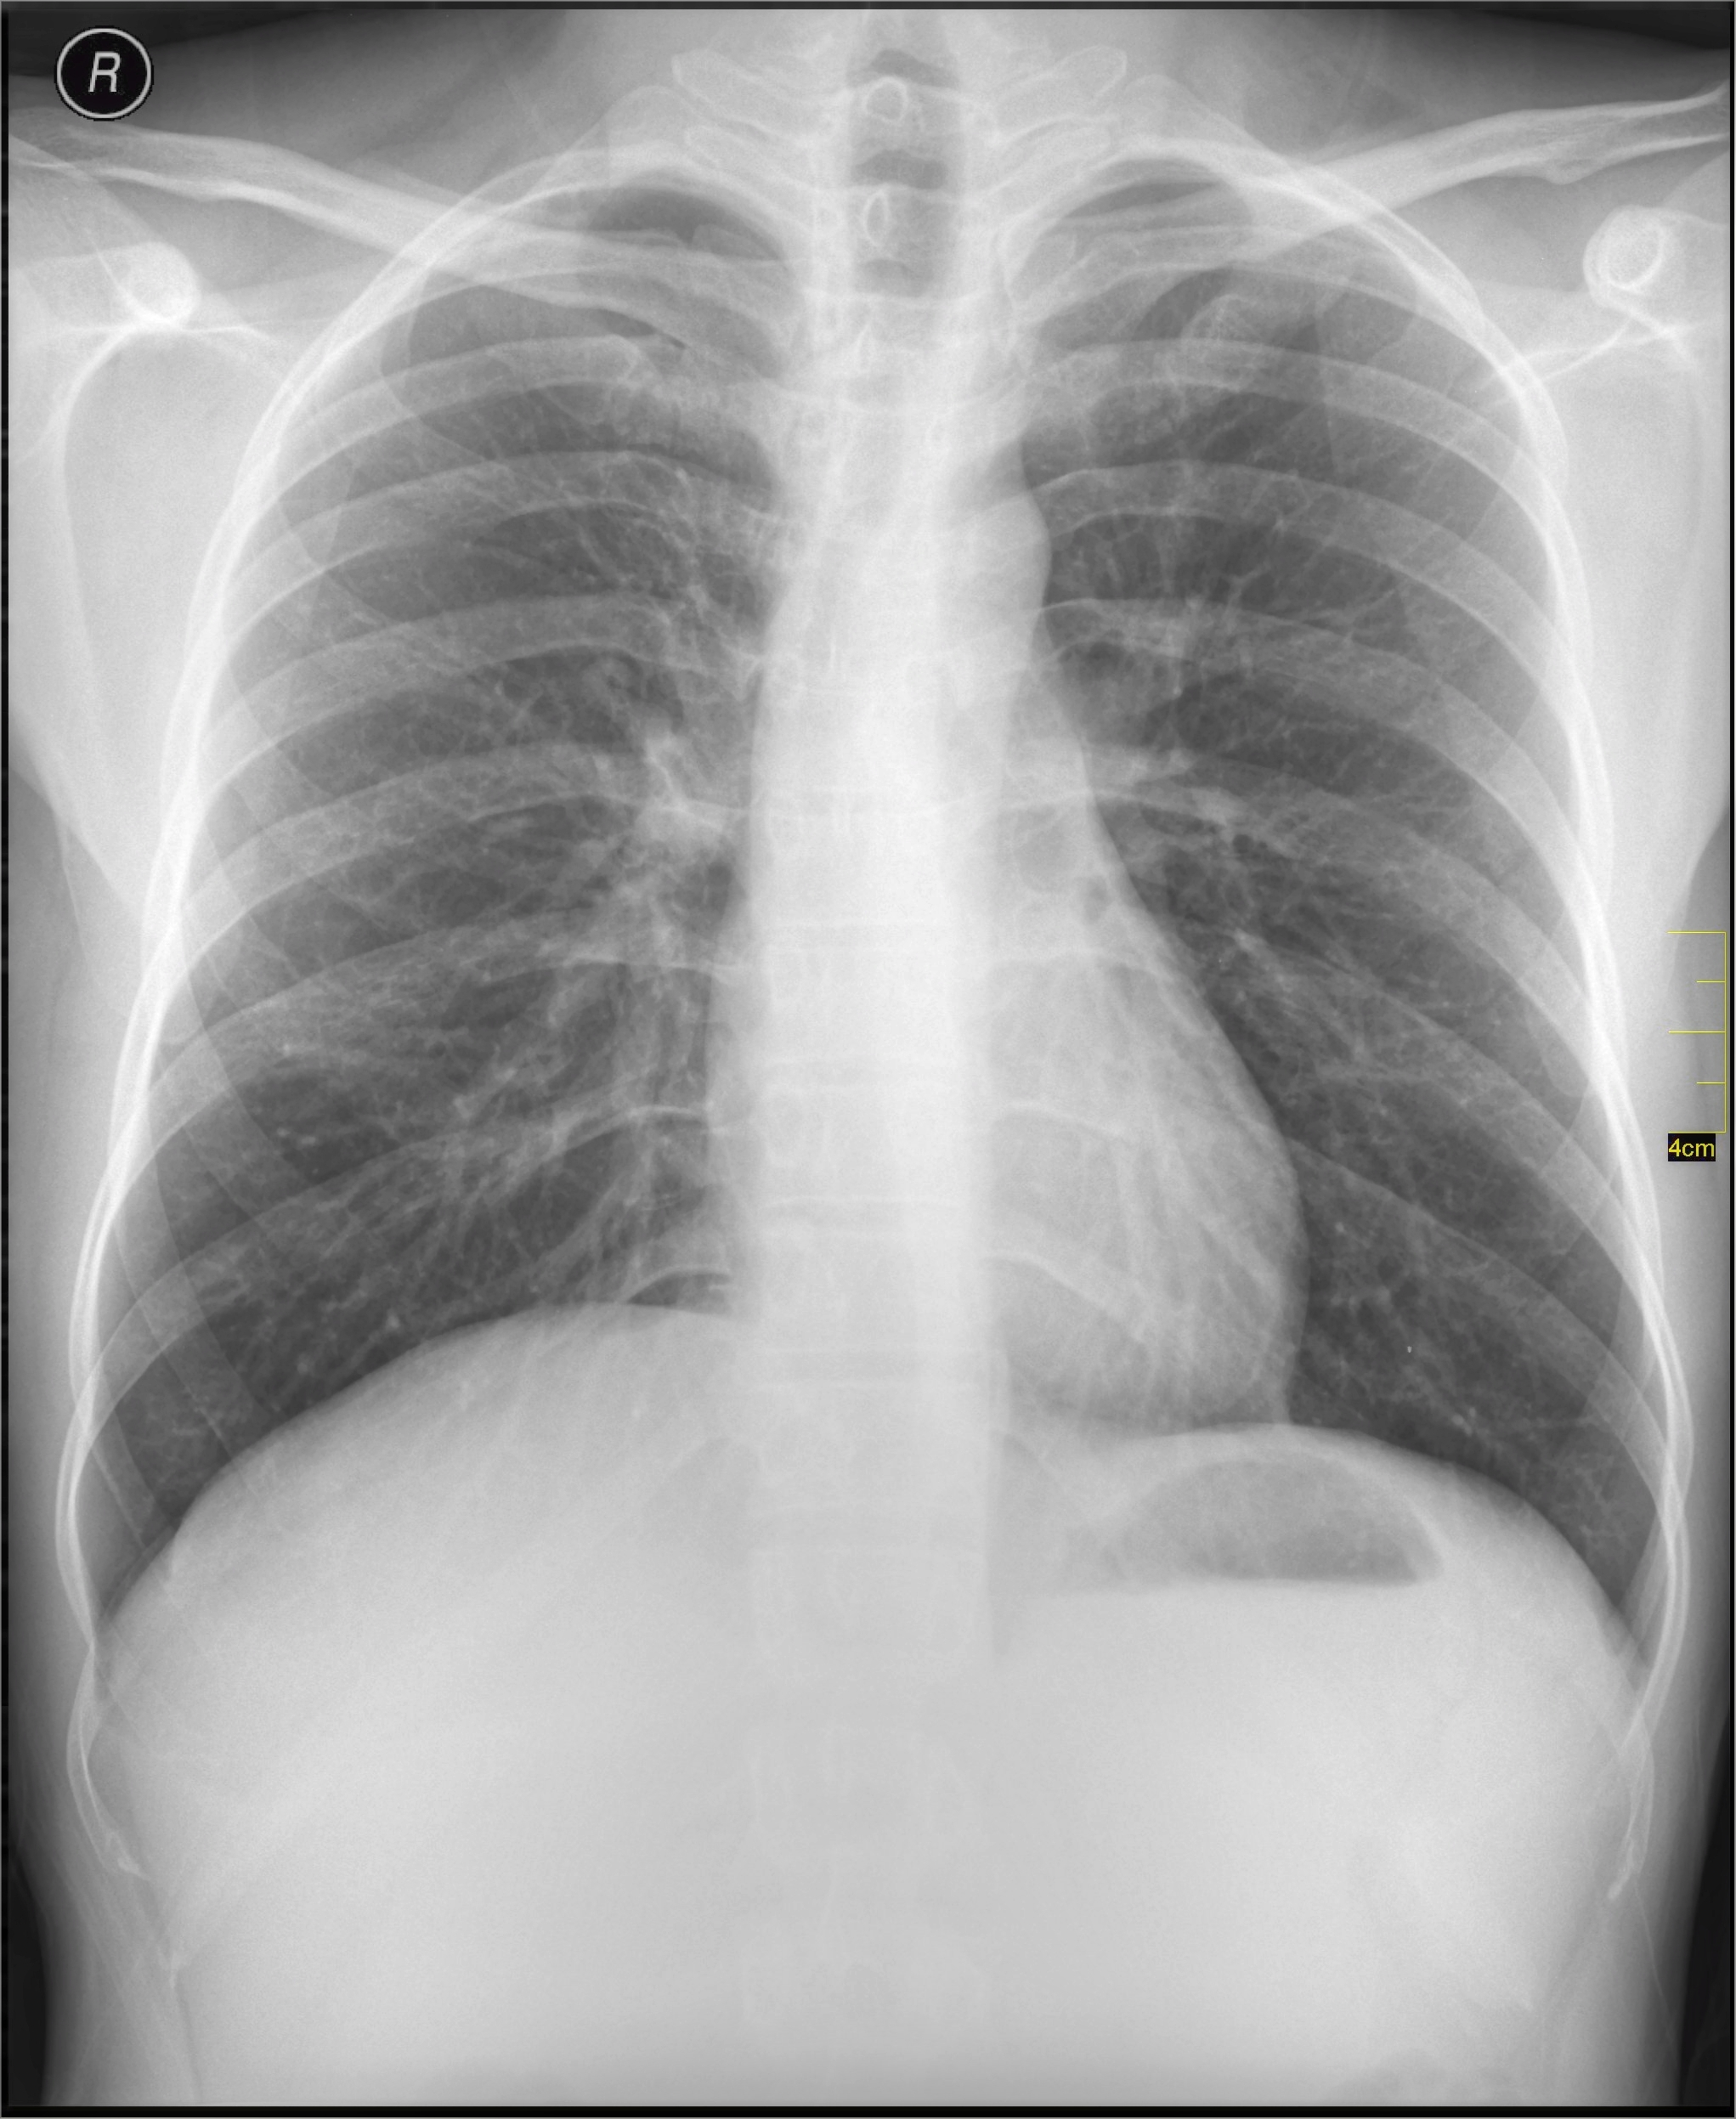
\includegraphics[scale = 0.065]{radio_thora.jpeg}
        \caption{Radiographie originale}
    \end{figure}
\end{frame}

\begin{frame}{Résultats - première méthode}
    \begin{figure}[t]
        \centering
        \begin{subfigure}[b]{0.35\textwidth}
            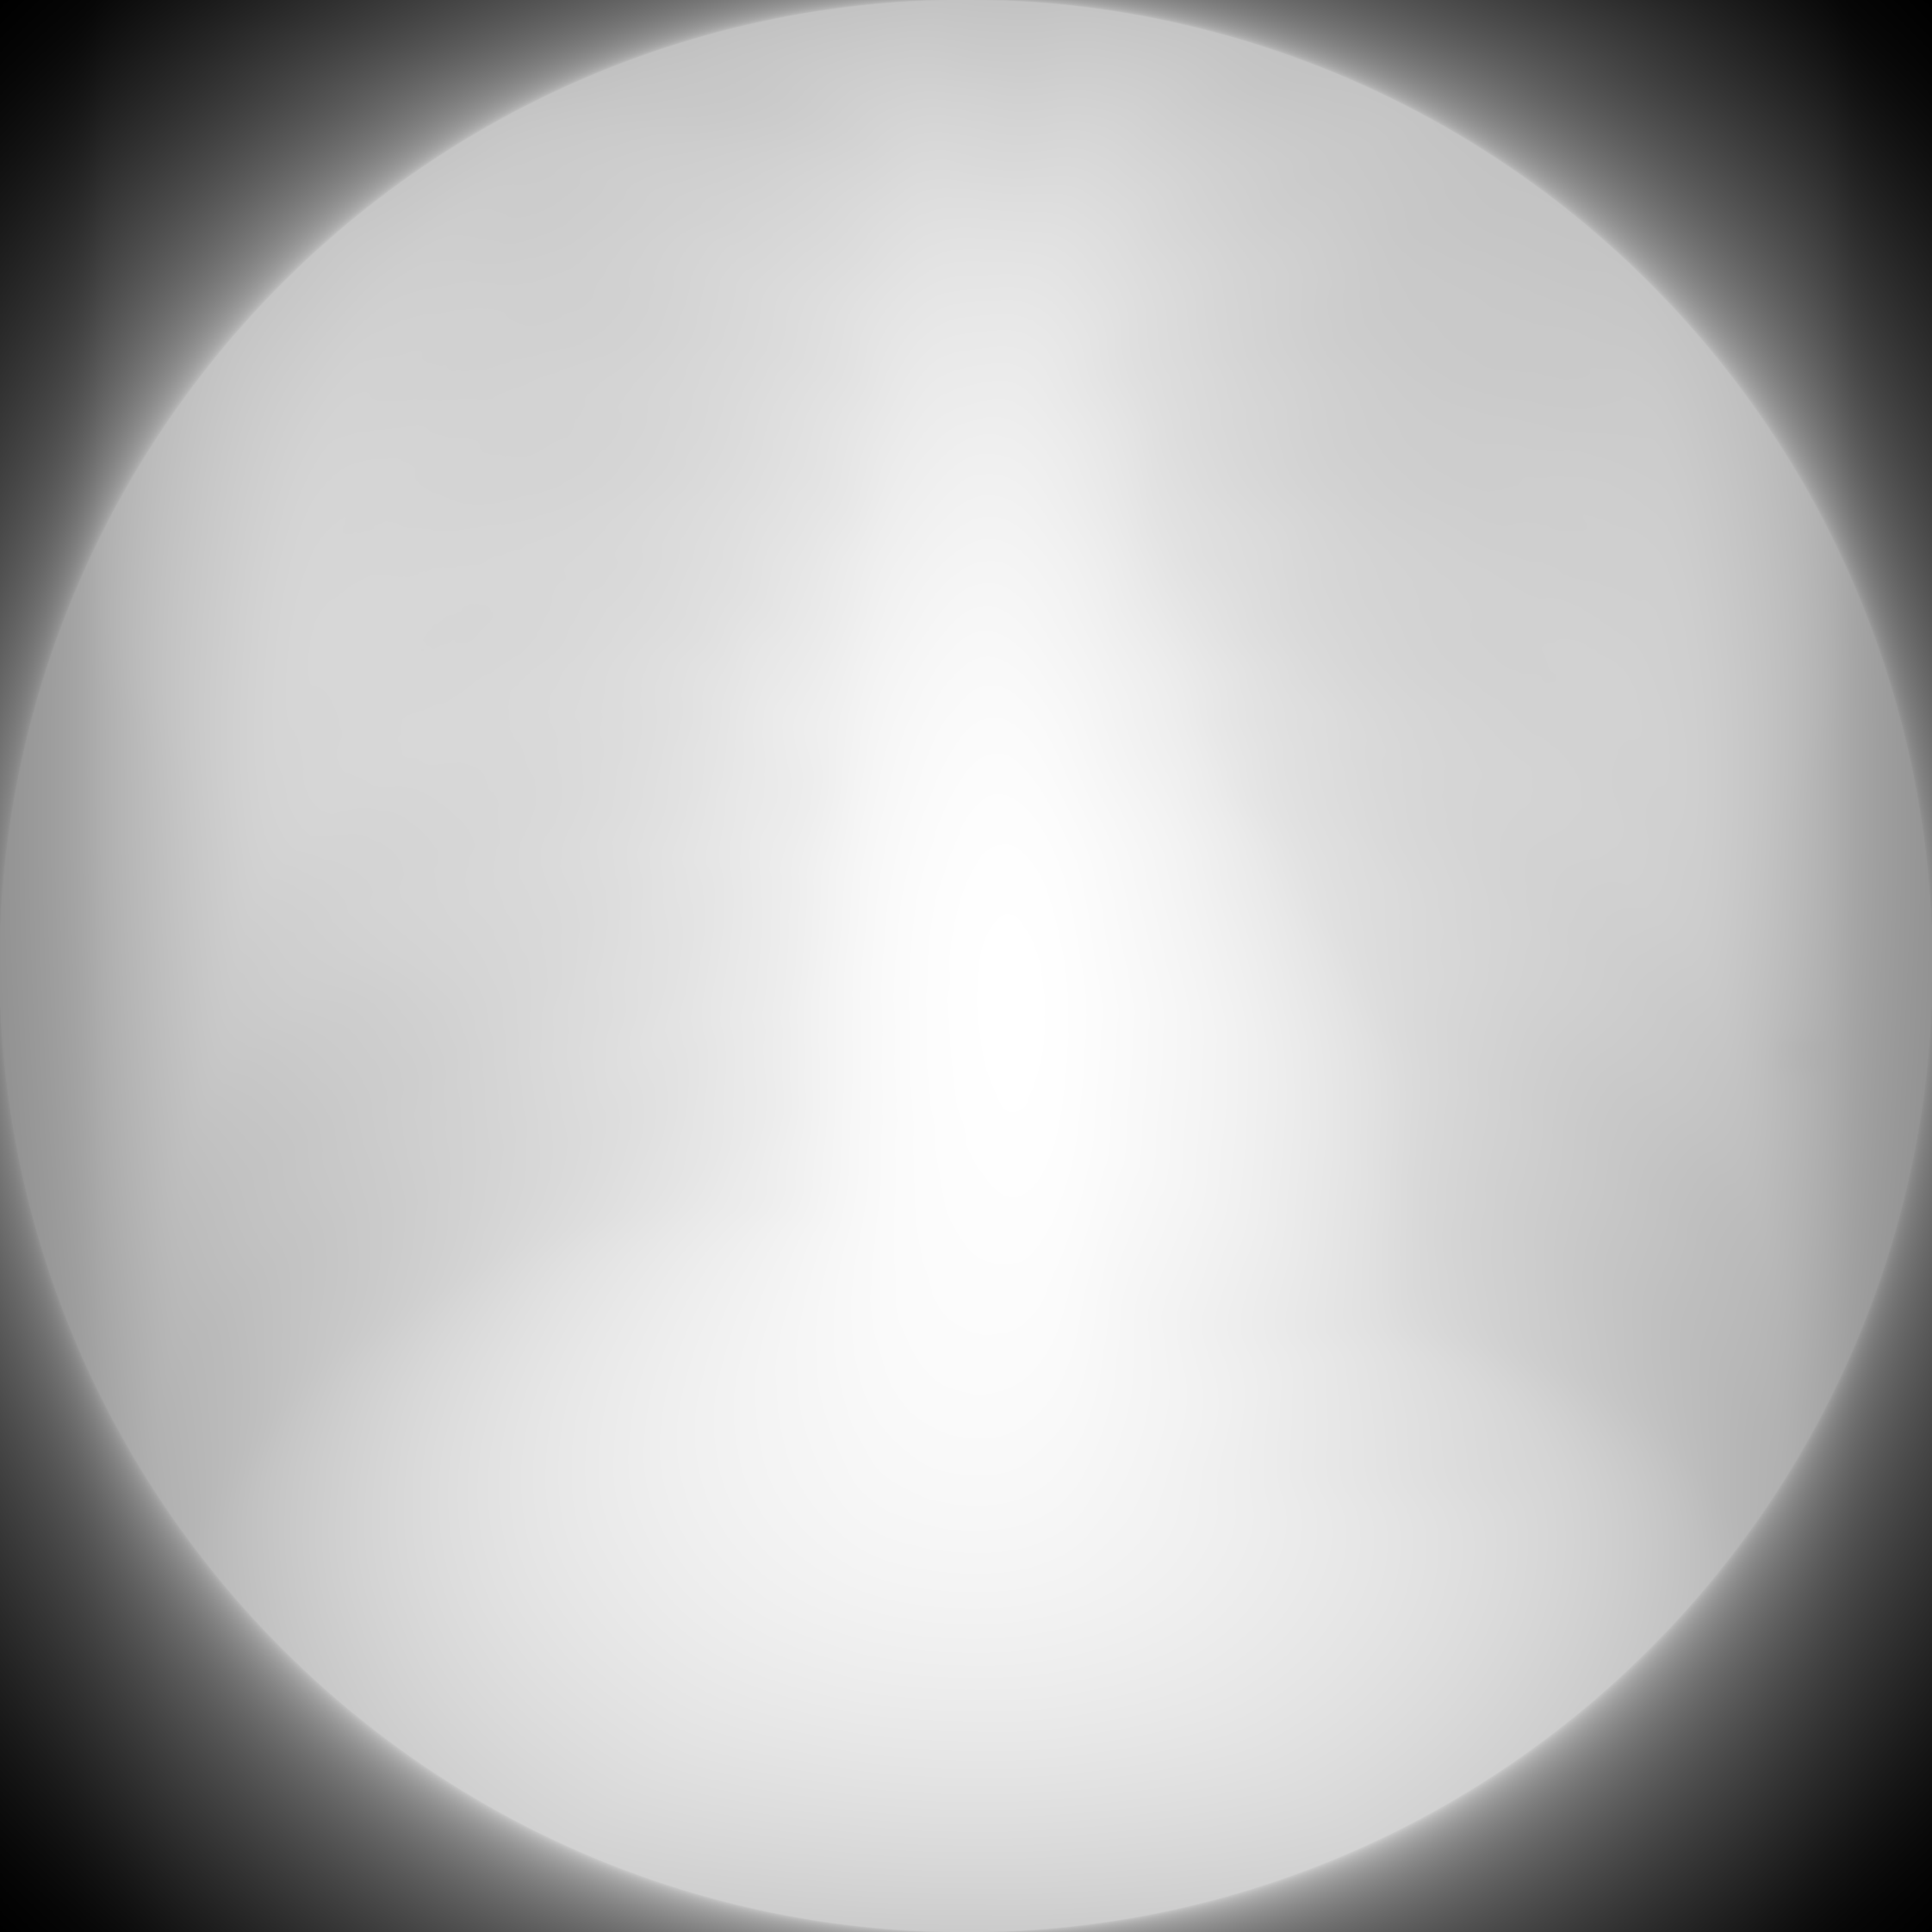
\includegraphics[width=\textwidth]{thoraSansFFT.png}
            \caption{Sans transformée de Fourier}
        \end{subfigure}
        \qquad \qquad 
        \pause
        \begin{subfigure}[b]{0.35\textwidth}
            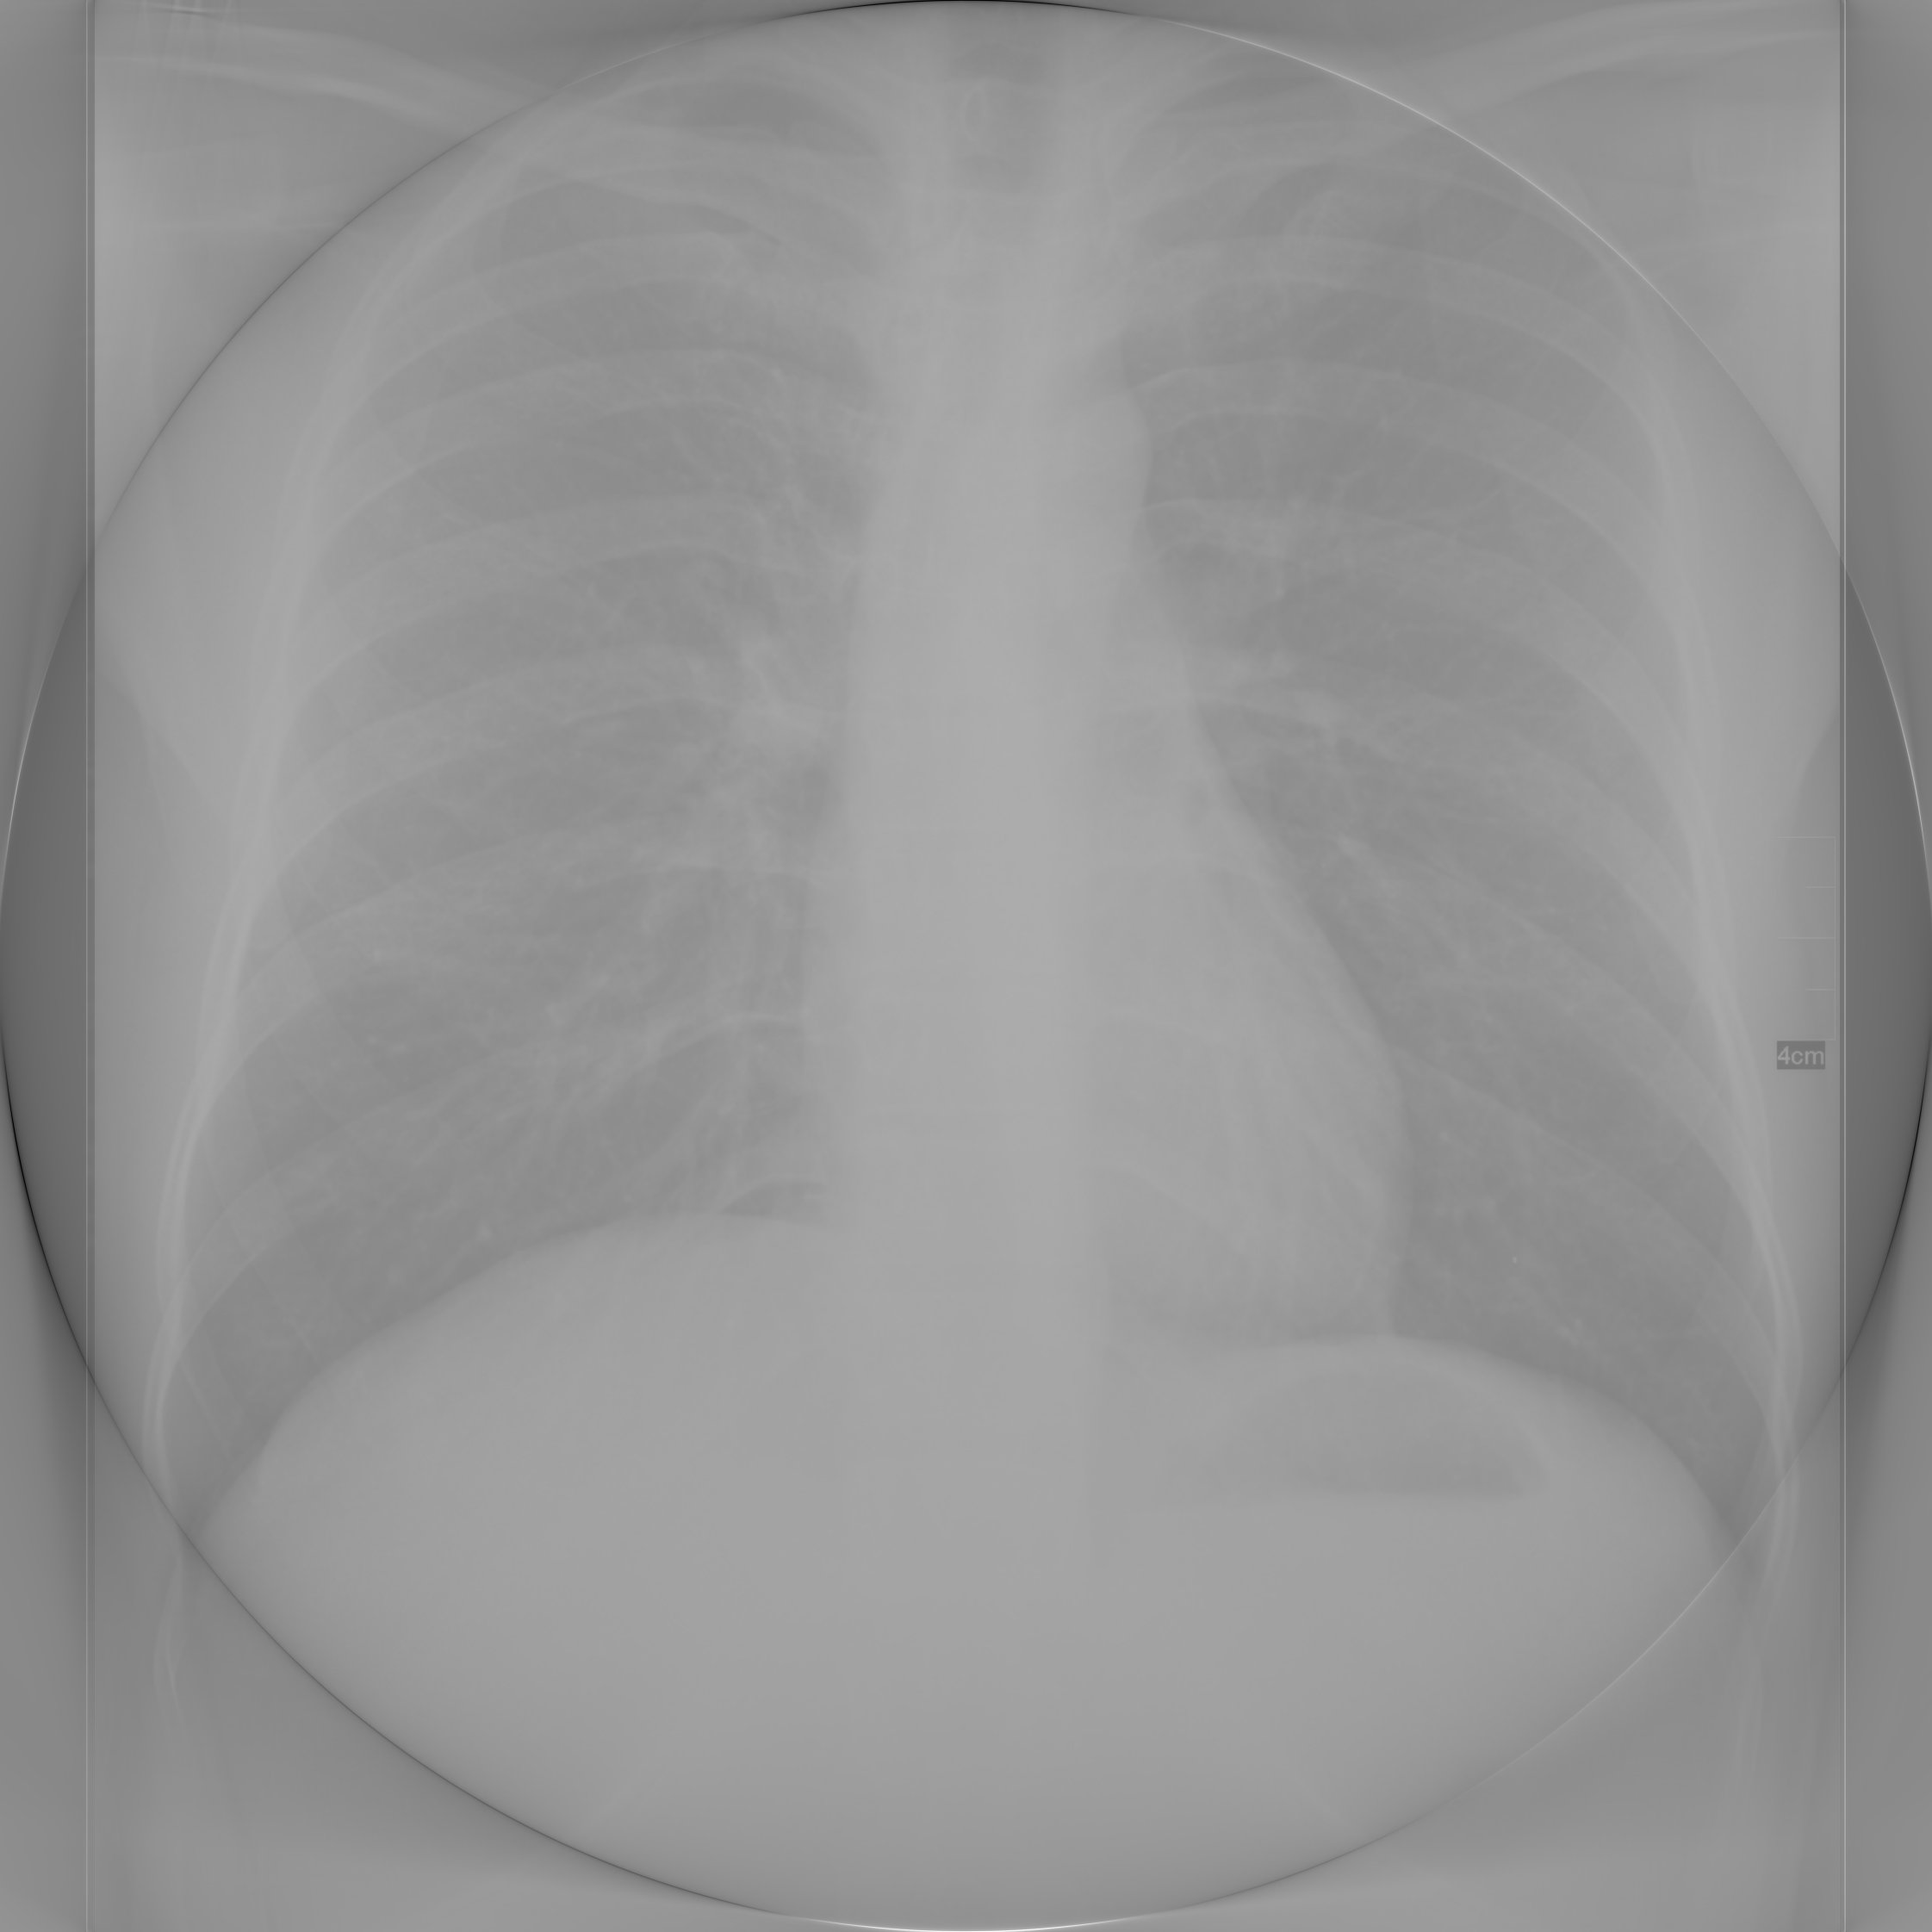
\includegraphics[width=\textwidth]{thoraxAvecFFT.png}
            \caption{Avec transformée de Fourier}
        \end{subfigure}
    \end{figure}
\end{frame}

\begin{frame}{Résultats - première méthode}
	\begin{figure}
        \centering
        \begin{tikzpicture}
            \begin{axis}[	grid= major ,
                width=0.8\textwidth ,
                xlabel = {taile de l'image (pixels)} ,
                ylabel = {temps d'execution (s)}]
                \addplot table {text.txt};
            \end{axis}
        \end{tikzpicture}
    \end{figure}
\end{frame}

\begin{frame}{Résultats - deuxième méthode}
    Un premier essai avec la matrice $R$ simple : 
    $$\forall (i,j) \in \iintervalle{1}{N} \times \iintervalle{1}{M},R_{i,j} = \left\{
        \begin{array}{ll}
            1 & \mbox{si le rayon } i \mbox{ passe par le pixel } j  \\
            0 & \mbox{sinon.}
        \end{array}
    \right.$$ 
    \pause
    \begin{itemize}
        \item images choisies : matrices aléatoires de taille $20 \times 20$
        \item 1000 projections
        \item itérations : de $3 000$ à $10 000 000$
    \end{itemize}
\end{frame}

\begin{frame}{Résultats - deuxième méthode}
    Reconstruction avec $3 000$ itérations
    \begin{figure}[t]
        \centering
        \begin{subfigure}[b]{0.35\textwidth}
            
\includegraphics[width=\textwidth]{matOriginale3.png}
            \caption{Matrice originale}
        \end{subfigure}
        \qquad \qquad 
        \pause
        \begin{subfigure}[b]{0.35\textwidth}
            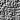
\includegraphics[width=\textwidth]{matReconstruction3.png}
            \caption{Matrice reconstruite}
        \end{subfigure}
    \end{figure}
Erreur maximale : 7.6729633974723335\\
Erreurs cumulées : 679.4563049009196
\end{frame}

\begin{frame}{Résultats - deuxième méthode}
    Reconstruction avec $100 000$ itérations
    \begin{figure}[t]
        \centering
        \begin{subfigure}[b]{0.35\textwidth}
            
\includegraphics[width=\textwidth]{matOriginale100.png}
            \caption{Matrice originale}
        \end{subfigure}
        \qquad \qquad 
        \pause
        \begin{subfigure}[b]{0.35\textwidth}
            
\includegraphics[width=\textwidth]{matReconstruction100.png}
            \caption{Matrice reconstruite}
        \end{subfigure}
    \end{figure}
Erreur maximale : 2.709169928559728\\
Erreurs cumulées : 191.0245806067057
\end{frame}

\begin{frame}{Résultats - deuxième méthode}
    Reconstruction avec $10 000 000$ itérations
    \begin{figure}[t]
        \centering
        \begin{subfigure}[b]{0.35\textwidth}
            
\includegraphics[width=\textwidth]{matOriginale10000.png}
            \caption{Matrice originale}
        \end{subfigure}
        \qquad \qquad 
        \pause
        \begin{subfigure}[b]{0.35\textwidth}
            
\includegraphics[width=\textwidth]{matReconstruction10000.png}
            \caption{Matrice reconstruite}
        \end{subfigure}
    \end{figure}
Erreur maximale : 0.006320163485931118\\
Erreurs cumulées : 0.2761238448059684
\end{frame}

\begin{frame}{Résultats - deuxième méthode}
	\begin{figure}
        \centering
        \begin{tikzpicture}
            \begin{axis}[	grid= major ,
                width=0.8\textwidth ,
                xlabel = {nombre d'itérations} ,
                ylabel = {erreurs cumulées}]
                \addplot table {text2.txt};
            \end{axis}
        \end{tikzpicture}
    \end{figure}
\end{frame}

\begin{frame}{Résultats - deuxième méthode}
	\begin{figure}
        \centering
        \begin{tikzpicture}
            \begin{axis}[	grid= major ,
                width=0.8\textwidth ,
                xlabel = {nombre d'itérations} ,
                ylabel = {erreur maximale}]
                \addplot table {text3.txt};
            \end{axis}
        \end{tikzpicture}
    \end{figure}
\end{frame}


\section{Annexe}
\subsection{La transformée de Fourier}
\begin{frame}{Transformée de Fourier}
    \begin{beamerboxesrounded}{Définitions}
        En dimension 1 : Soit $f : \R \longmapsto \R$ une fonction intégrable on définit la transformée de Fourier par : 
        $$\forall \nu \in \R, \; \widehat{f}(\nu) = \int_{\R} f(t)\mathrm{e}^{-2 i \pi \nu t } \dd t$$  
        En dimension 2 : Soit $f : \R^2 \longmapsto \R$ une fonction intégrable on définit la transformée de Fourier par : 
        $$\forall (u,v) \in \R^2, \; \widehat{f}(u,v) = \int_{\R^2} f(x,y) \mathrm{e}^{-2 i \pi (ux + vy)} \dd x \dd y $$
    \end{beamerboxesrounded}
\end{frame}
\begin{frame}{Transformée de Fourier}
    \begin{beamerboxesrounded}{Théorème d'inversion de Fourier}
        Sous certaines hypothèses supposées vérifiées dans le cadre de notre étude on peut accéder à $f$ par inversion de sa transformée de Fourier.  \\
        En dimension 1 : $$\forall t \in \R, f(t) = \int_{\R} \widehat{f}(\nu)\mathrm{e}^{2i\pi \nu t} \dd \nu$$
        En dimension 2 : $$\forall (x,y) \in \R^2, f(x,y) = \int_{\R^2} \widehat{f}(u,v)\mathrm{e}^{2i\pi (ux + vy)} \dd u \dd v$$
    \end{beamerboxesrounded}
Il est par exemple suffisant que $f$ soit dans l'espace de Schwartz $\mathcal{S}(\R^d) \; (d \in \{1,2\})$ où : 
$$\mathcal{S}(\R) = \{f \in \mathcal{C}^{\infty} : \forall (n,m) \in \N, x \mapsto x^{n} f^{(m)}(x) \text{ bornée} \}$$
$$\mathcal{S}(\R^2) = \{f \in \mathcal{C}^{\infty} : \forall (p,q,n,m) \in \N^4, (x,y) \mapsto x^{p}y^q \partial_x^n \partial_y^m f(x,y) \text{ bornée}\}$$
\end{frame}
\subsection{La transformée de Fourier discrète}
\begin{frame}{Transformée de Fourier discrète}
    \begin{beamerboxesrounded}{Transformée de Fourier discrète}
        Soit $f$ une fonction estimée aux points $(u_1, ... , u_N)$ on définit la transformée de Fourier discrète (TFD) de $f$ par la suite $(F(u_1), ... , F(u_N))$
        où : $$\forall k \in \iintervalle{1}{N}, \; F(u_k) = \sum_{l = 1}^N f(u_l)\exp\left(\frac{-2i\pi k l}{N}\right)$$
    \end{beamerboxesrounded}
    \begin{beamerboxesrounded}{Expression matricielle}
        $$\begin{pmatrix}
            F(u_1) \\
            \vdots \\
            F(u_N)
        \end{pmatrix} =
            \Omega
          \begin{pmatrix}
             f(u_1) \\ \vdots \\ f(u_N)
         \end{pmatrix}\\
         \text{ avec } \Omega = (\omega^{kl})_{(k,l)} \text{ et } \omega = \mathrm{e}^{\frac{-2i\pi}{N}}$$
    \end{beamerboxesrounded}
\end{frame}
\begin{frame}{Transformée de Fourier discrète}
    \begin{beamerboxesrounded}{Spécificité de la matrice $\Omega$}
        La matrice $\frac{\Omega}{\sqrt{N}}$ est dite unitaire. 
    \end{beamerboxesrounded}
    $ \text{Soient } k,l \in \iintervalle{1}{N}$, 
    $$[\Omega^* \Omega]_{k,l} = \sum_{d = 1}^N [^t\overline{\Omega}]_{k,d} [\Omega]_{d,l} = \sum_{d = 1}^N \omega^{-kd} \omega^{dl} = \sum_{d= 1}^N \omega^{d(l-k)} = \delta_{k,l}N$$
    Donc : $$\left(\frac{\Omega}{\sqrt{N}}\right)^* \frac{\Omega}{\sqrt{N}} = I_N$$
    Conséquences : $\Omega$ est inversible et s'inverse facilement
\end{frame}

\begin{frame}{Transformée de Fourier discrète}
    \begin{beamerboxesrounded}{Transformée de Fourier discrète - dimension 2}
        Soit $f$ une fonction estimée aux points $(u_1, ... , u_N, v_1, ... , v_M)$ on définit la transformée de Fourier discrète 2D de $f$ par la suite double $(F(u_1, v_1), F(u_1, v_2), ... , F(u_N,v_M))$ où : 
        $$\forall k, l \in \iintervalle{1}{N} \times \iintervalle{1}{M}, F(u_k, u_l) = \sum_{n = 1}^N \sum_{m = 1}^M f(u_n,u_m) \mathrm{e}^{\frac{-2i \pi k n}{N}} \mathrm{e}^{\frac{-2i \pi l m}{M}} $$
    \end{beamerboxesrounded}
\end{frame}

\subsection{Code Python : méthode par la transformée de Fourier discrète}
\begin{frame}[fragile, allowframebreaks]{Annexe - Code méthode par la transformée de Fourier discrète}
\lstinputlisting{TIPE_v3.py}
\end{frame}

\subsection{Code Python : méthode ART}

\begin{frame}[fragile, allowframebreaks]{Annexe - Code méthode ART}
    \begin{lstlisting}
from math import cos, sin, sqrt, pi
import numpy as np
import matplotlib.pyplot as plt

mat = np.random.randint(10, size=(20, 20))
l = mat.shape[0]  # nombre de ligne (coordonnee y)
L = mat.shape[1]  # nombre de colonne (coordonne x)
M = l * L
d = sqrt(l ** 2 + L ** 2)

# donne le point d'intersection de deux droites donnees en polaire
def distance(point1, point2):
    return sqrt((point1[0] - point2[0]) ** 2 + (point1[1] - point2[1]) ** 2)


# produit scalaire canonique
def ps(m1, m2):
    return float((sum([i * j for (i, j) in zip(m1, m2)])))


# coordonnees du pixel j
def pixel(j):
    r = (j - 1) % L  # reste dans la division euclidienne de j-1 par L
    q = (j - 1) // L  # quotient dans la division euclidienne de j-1 par L
    return (q, r)


# conversion de l'image en une matrice colonne :
def colonne():
    m = np.zeros((M, 1))
    for j in range(0, M):
        (q, r) = pixel(j + 1)
        m[j, 0] = mat[q, r]
    return m


# equation polaire de la droite
def rayon(u, t, theta):
    return (u * sin(theta) + t * cos(theta), u * cos(theta) - t * sin(theta))


# est ce que la droite de parametres (u,theta) passe par le pixel j

def isInPixel(u, theta, j):
    (a, b) = pixel(j)
    if theta != 0 and theta != pi / 2:
        # Cas 1 (haut) :
        t = (a - u * sin(theta)) / cos(theta)
        y2 = rayon(u, t, theta)[1]
        if b <= y2 <= b + 1:
            return True
        # Cas 2 (bas) :
        t = (a + 1 - u * sin(theta)) / cos(theta)
        y2 = rayon(u, t, theta)[1]
        if b <= y2 <= b + 1:
            return True
        # Cas 3 (gauche):
        t = (u * cos(theta) - b) / sin(theta)
        x2 = rayon(u, t, theta)[0]
        if a <= x2 <= a + 1:
            return True
        # Cas 4 (droite):
        t = (u * cos(theta) - b - 1) / sin(theta)
        y2 = rayon(u, t, theta)[0]
        if a <= x2 <= a + 1:
            return True
    elif theta == 0:
        if a <= u <= a + 1:
            return True
    elif theta == pi / 2:
        if b <= u <= b + 1:
            return True
    return False


def intersection(u, theta, j):
    long = 0
    if not isInPixel(u, theta, j):
        return False
    (a, b) = pixel(j)
    if theta != pi / 2 and theta != 0:
        lst = []
        lst2 = []
        # intersection avec le bord gauche :
        t = (u * cos(theta) - b) / sin(theta)
        lst.append(rayon(u, t, theta))

        # intersection avec le bord droit :
        t = (u * cos(theta) - b - 1) / sin(theta)
        lst.append((rayon(u, t, theta)))

        # intersection avec le bord haut :
        t = (a - u * sin(theta)) / cos(theta)
        lst.append((rayon(u, t, theta)))

        # intersection avec le bord bas :
        t = (a + 1 - u * sin(theta)) / cos(theta)
        lst.append((rayon(u, t, theta)))
        for point in lst[0:2]:
            if a <= point[0] <= a + 1:
                lst2.append(point)
        for point in lst[2:4]:
            if b <= point[1] <= b + 1:
                lst2.append(point)
        assert len(lst2) == 2
        long = distance(lst2[0], lst2[1])
    else:
        long = 1
    return long


# definition des rayons de projections
def projections(nb_dir, nb_droite):
    dir = np.linspace(0, pi / 2, nb_dir)
    droite = np.linspace(5, 15, nb_droite)
    proj = []
    for theta in dir:
        for u in droite:
            proj.append((u, theta))
    return proj


def matR_v1(proj):
    N = len(proj)
    R = np.zeros((N, M))
    for i in range(1, N + 1):
        for j in range(1, M + 1):
            if isInPixel(proj[i - 1][0], proj[i - 1][1], j):
                R[i - 1, j - 1] = 1
    return R


# definition de la matrice R - version 2
def matR_v2(proj):
    N = len(proj)
    R = np.zeros((N, M))
    for i in range(1, N + 1):
        for j in range(1, M + 1):
            R[i - 1, j - 1] = intersection(proj[i - 1][0], proj[i - 1][1], j)
    return R


# construction de la matrice de projection
def matP(R):
    m = colonne()
    N = R.shape[0]
    P = np.zeros((N, 1))
    for i in range(0, N):
        for j in range(0, M):
            P[i, 0] += R[i, j] * m[j, 0]
    return P


# On peut alors tenter de resoudre le probleme inverse : RF = P (par n iteration)
def operateurs(R):
    # extractions des lignes de la matrice R
    N = R.shape[0]
    lignes = []
    transpo = []
    q = []
    for i in range(N):
        lignes.append(R[i, :])
        Ni = np.transpose(np.array([R[i, :]]))
        transpo.append(Ni)
        q.append(P[i, 0] * Ni / ps(Ni, Ni))

    # definition des operateurs de projections orthognales
    operator = []
    id = np.eye(M)
    for i in range(N):
        Ni = transpo[i]
        Ti = id - (1 / ps(Ni, Ni)) * np.dot(Ni, np.transpose(Ni))
        operator.append(Ti)
    return [q, operator]


def reconstruction(n, op, F_0=np.zeros((M, 1))):
    nb = len(op[0])
    T = op[1]
    q = op[0]
    F = F_0
    for k in range(1, n):
        F = q[(k - 1) % nb] + np.dot(T[(k - 1) % nb], F - q[(k - 1) % nb])
    return F


proj = projections(500, 100)
R = matR_v1(proj)
P = matP(R)
op = operateurs(R)
FC = reconstruction(500, op)


def columnIntoMatrix(C):
    A = np.zeros((l, L))
    for i in range(l):
        for j in range(L):
            A[i, j] = C[i * L + j, 0]
    return A
F = columnIntoMatrix(FC)
plt.imshow(F)
plt.show()
plt.imshow(mat)
plt.show()
    \end{lstlisting}
\end{frame}
\end{document}